\documentclass[10pt, landscape, a4paper]{article}
\usepackage{geometry}[landscape]
\usepackage{multicol}
\usepackage{graphicx}
\usepackage{amsmath} 
\usepackage{amssymb}
\usepackage{ccicons}
\usepackage{hyperref}

\usepackage[dvipsnames]{xcolor}

% Set page margins
\geometry{top=.8cm, left=.8cm, right=.8cm, bottom=.8cm}

% Set paragraph indentation
\setlength{\parindent}{0pt}

% Set path for assets
\graphicspath{{assets/}}

\setlength{\columnsep}{20pt}
\raggedcolumns

% _____ CUSTOM COMMANDS __________________________________________
\newcommand{\E}[0]{\mathbb{E}}
\newcommand{\R}[0]{\mathbb{R}}

\newcommand{\sgn}[0]{\text{sgn}}

\newcommand{\argmin}[1]{\underset{#1}{\text{argmin}}}
\newcommand{\argmax}[1]{\underset{#1}{\text{argmax}}}

\begin{document}
\begin{multicols*}{3}

% _____ CONTENT __________________________________________________

% main heading
\begin{center}
	\Large{\textbf{Visual Computing}} \\
    \small{by dcamenisch}
\end{center}

\section{Introduction}

This document is a summary of the 2022 edition of the lecture \textit{Visual Computing} at ETH Zurich. I do not guarantee correctness or completeness, nor is this document endorsed by the lecturers. If you spot any mistakes or find other improvements, feel free to open a pull request at \url{https://github.com/DannyCamenisch/vc-summary}. This work is published as CC BY-NC-SA.
\begin{center}
	\ccbyncsa
\end{center}

\begin{center}
	\Large{\textbf{Computer Vison}}
\end{center}

\section{The Digital Image}

An image is simply a continuous function over 2 or 3 variables (XY-coordinates and possibly time). Usually we use brightness as the value of the function, but other physical values can also be used. For a computer this is just a collection of numbers, but instead of continuous values we have discrete. Note that in real life images are never completely random and almost always contain some structure. It is important to know that \textbf{pixels are not little squares}, they are point measurements.

When taking a picture with a digital camera, we can encounter various problems, e.g.:
\begin{itemize}
	\item Transmission Interference
	\item Compression Artefacts
	\item Spilling
	\item Sensor Noise
\end{itemize}

\subsection{Sampling}

When taking an image, we are sampling such a continuous. When trying to reconstruct the original function, we can encounter undersampling, i.e. when we loose information due to a too low amount of sampling points. 

\begin{center}
	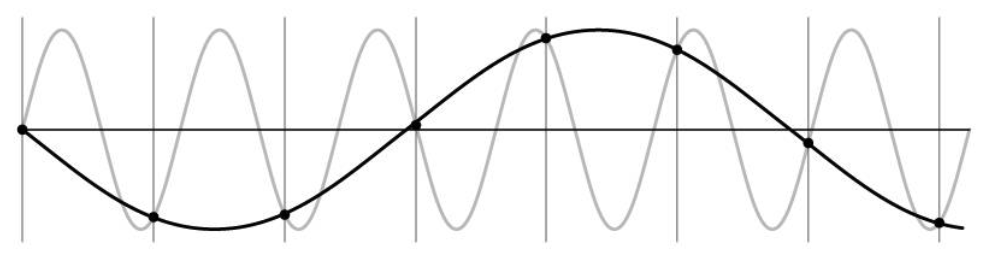
\includegraphics[width=0.8\linewidth]{undersampling.png}
\end{center}

Due to undersampling, the result can not be distinguished from a lower or a higher frequency wave. Signal disguised as other frequencies is also called \textbf{aliasing}. \medskip

\textbf{Nyquist-Shannon Sampling Theorem}

For sine waves we have to sample at half the wave length. This corresponds to double the frequency, we also call this the \textbf{Nyquist Frequency}.

\subsection{Quantization}

Another problem we have to deal with is \textbf{quantization}, since the real valued function will get digital (integer) values, it is lossy. Compared to sampling which lets us reconstruct the original function. Simple quantization uses equally spaced levels with $k$ intervals.

\begin{center}
	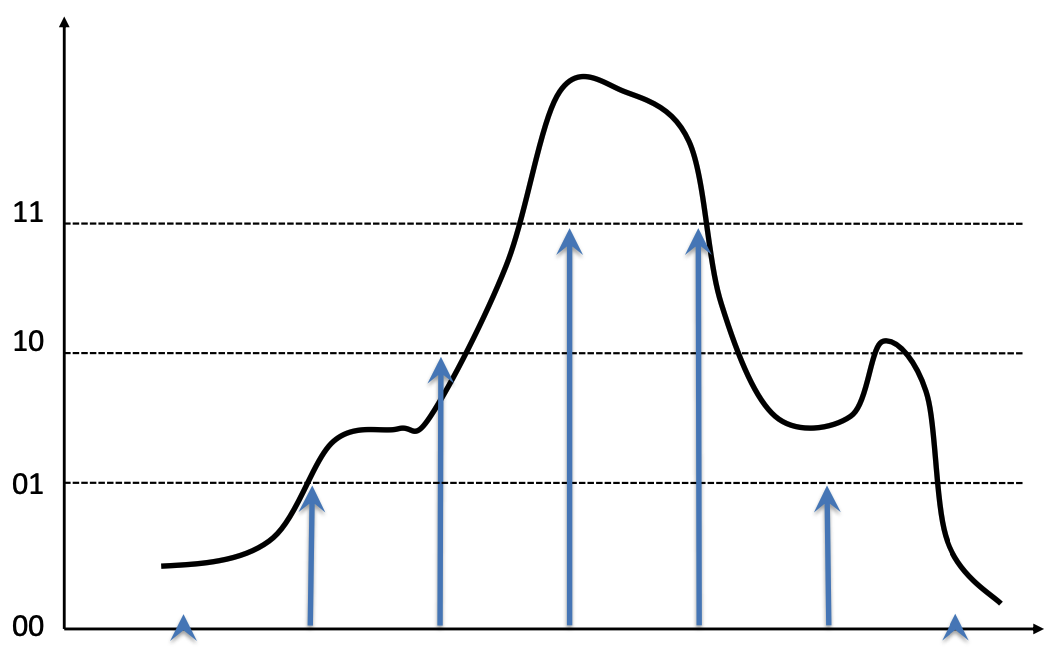
\includegraphics[width=0.8\linewidth]{quantization.png}
\end{center}

\subsection{Image Properties}

Image resolution is divided into two parts:
\begin{itemize}
	\item Geometric Resolution: How many pixels per area
	\item Radiometric Resolution: How many bits per pixel
\end{itemize}

\subsection{Noise}

When taking pictures we can almost always encounter some noise. A common way to model this is additive gaussian noise:
$$I(x,y) = f(x,y) + c, \qquad c \sim \mathcal N(0, \sigma^2)$$

The signal to noise ratio (SNR) is an index of image quality:
$$\text{SNR} = \frac{F}{\sigma}, \qquad F = \frac{1}{XY} \sum_{x=1}^{X}\sum_{y=1}^{Y} f(x,y)$$

The usefulness for this metric can vary drastically depending on the type of image (dark images will have a higher SNR compared to bright images). Therefore we introduce peak SNR:
$$\text{PSNR} = \frac{F_\text{max}}{\sigma}$$
\section{Segmentation}

Image segmentation is often viewed as the ultimate classification problem, once solved, computer vision is solved. A complete segmentation of an image is a finite set of disjunct regions $R_1, ..., R_n$, such that $I = \bigcup R_i$.


\subsection{Thresholding}

Thresholding is a simple segmentation process, that produces a binary image by labelling each pixel in or out of the region of interest. We do this by comparison of the grey level with a threshold value $T$. Another, better approach can be chromakeying. Hereby we measure the distance from a defined color $g$:

$$I_\alpha = |I - g| > T$$

One limit of thresholding is that it does not consider image context.


\subsection{Segmentation Performance}

If we want to choose the best performing segmentation algorithm or determine a good value for $T$, we need a performance metric. To use automatic analysis, one needs to know the true classification of each test, for this the test images have to be segmented by hand. \medskip

One performance metric is the ROC curve. This curve characterizes the error trade-off in binary classification tasks, by plotting the true positive fraction against the false positive fraction. We often choose the operating point on the ROC curve, by assigning cost and values to each outcome:
\begin{itemize}
	\item $V_{\text{TN}}$ - value of true negative
	\item $V_{\text{TP}}$ - value of true positive
	\item $C_{\text{FN}}$ - cost of false negative
	\item $C_{\text{FP}}$ - cost of false positive
\end{itemize}

We then choose the point on the ROC curve with the gradient:
$$\beta = \frac{N}{P} \cdot \frac{V_{\text{TN}} + C_{\text{FP}}}{V_{\text{TP}} + C_{\text{FN}}}$$


\subsection{Pixel Connectivity}

We try to define which pixels are neighbors.

\begin{center}
	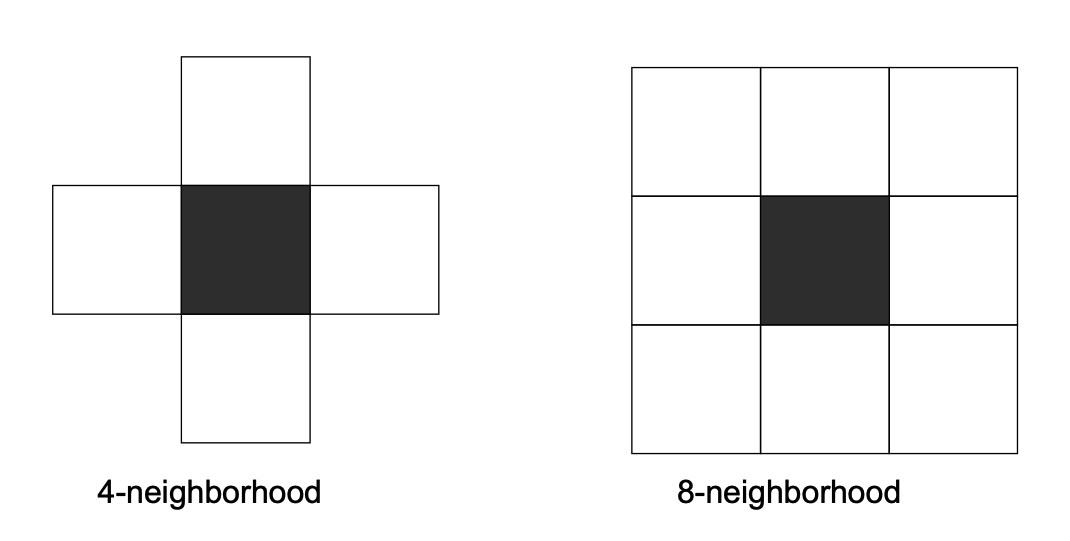
\includegraphics[width=\linewidth]{pixel-neighborhoods.png}
\end{center}

A 4 (or 8) connected path between $p_1, p_n$ is a set of pixels such that every $p_i$ is a 4 (or 8) neighbor of $p_{i+1}$. Now we can defined a region as 4 (or 8) connected if it contains a 4 (or 8) connected path between any two of its pixels.

With this we can introduce \textbf{region growing}. We start from a seed point or region and add neighboring pixels that satisfy the criteria defining a region until we can include no more pixels. There are different approaches to selecting the seed and we could also use multiple seeds. For the inclusion criteria we could choose thresholding or a distribution model.

Another criteria is a snake (active contour). While each point along the contour moves away from the seed, it always has to have some smoothness constraints (minimizing energy function).


\subsection{Distance Measures}

Plain background substraction $I_\alpha = |I - I_{bg}| > T$, where $I_{bg}$ is the background image, we get this by fitting a Gaussian (Mixture) model per pixel. Even better would be:
$$I_\alpha = \sqrt{(I - I_{bg})^\top \Sigma (I - I_{bg})} > T$$

Where $\Sigma$ is the background pixel appearance covariance matrix.


\subsection{Markov Random Fields}

We can add spatial relations with Markov Random Fields (2D Markov Chains).

\begin{center}
	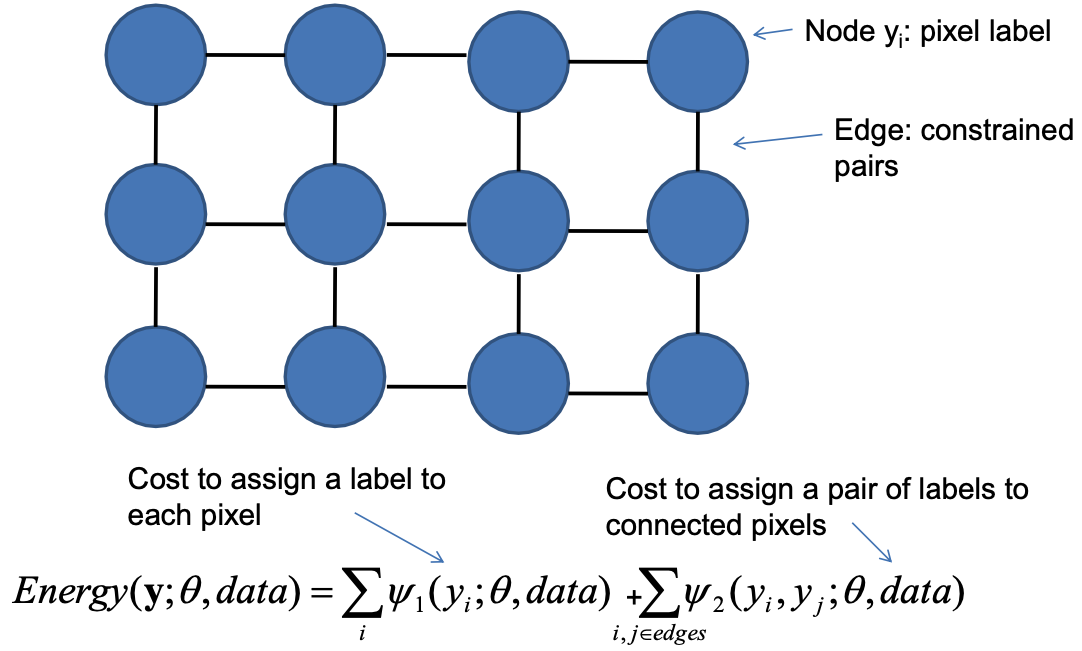
\includegraphics[width=\linewidth]{markov-field.png}
\end{center}

Using a graph cut algorithm we can determine the optimal segementation. We can further optimize this by using iterated graph cut and k-means for learning the colour distribution (GMM) of the image.

\begin{center}
	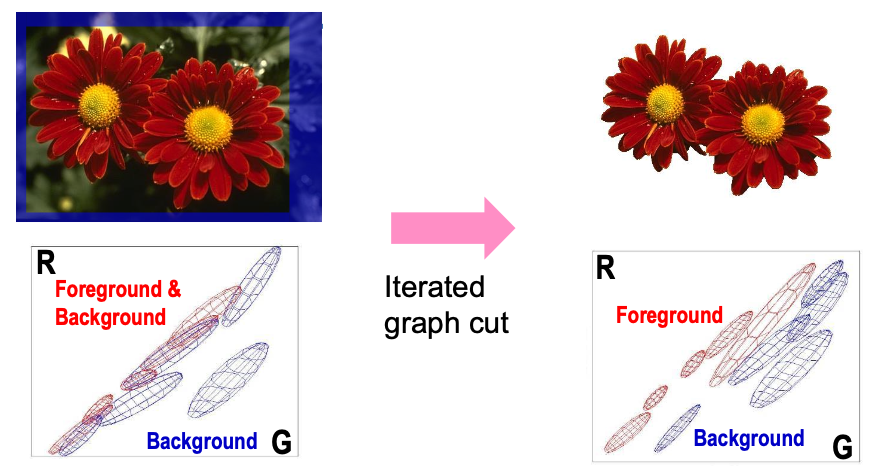
\includegraphics[width=\linewidth]{iterated-graph-cut.png}
\end{center}

\section{Convolution and Filtering}

Convolution and filtering are some of the most basic operations of image processing. 


\subsection{Filtering}

Image filtering is the process of modifying pixels in an image base on some function of a local neighborhood of the pixel.

\subsubsection{Linear Shift-Invariant Filtering}

Linear lhift-invariant filtering means using linear combinations of neighbors and doing the same for each pixel (shift-invariant). These filters are often used for low-level image processing, smoothing / noise reduction, sharpening and feature detection. Linear operations can be written as:
$$I'(x,y) = \sum_{(i,j) \in N(x,y)} K(x,y; i, j) I(x,y)$$

Here $I$ is the input image, $I'$ the output image, $K$ is the kernel and $N$ is the neighborhood. Operations are shift-invariant if $K$ does not depend on $(x,y)$.


\subsection{Correlation}

Correlation, e.g. template matching:

\begin{center}
	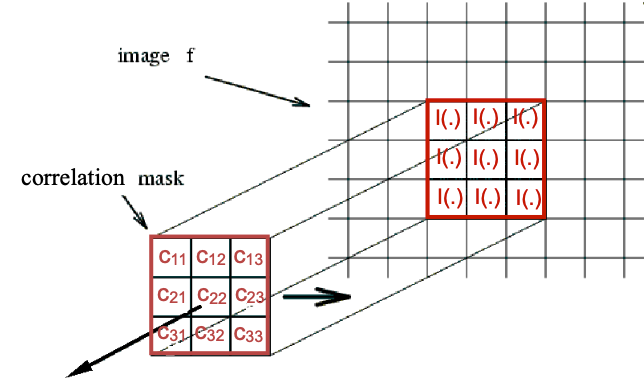
\includegraphics[width=0.9\linewidth]{correlation.png}
\end{center}
$$I' = K \circ I, \quad I'(x,y) = \sum_{(i,j) \in N(x,y)} K(i, j) I(x + i, y + j)$$

Correlation takes an input image and a weight mask, then each pixel gets "replaced" by the weighted sum of its neighborhood. This can be described as taking multiple input location and writing one output location.


\subsection{Convolution}

Convolution, e.g. point spread function:

\begin{center}
	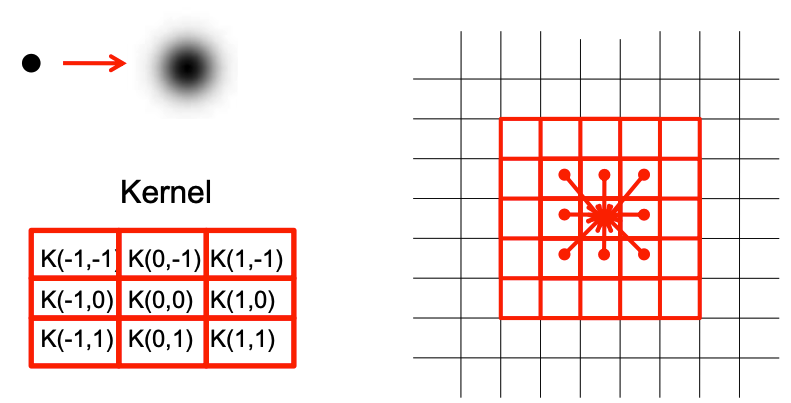
\includegraphics[width=0.9\linewidth]{convolution.png}
\end{center}
$$I' = K * I, \quad I'(x,y) = \sum_{(i,j) \in N(x,y)} K(i, j) I(x - i, y - j)$$

This is similar to the correlation, but \textbf{the kernel is reversed}. This can be described as taking one input location and writing multiple output location, the opposite of the correlation. By default we use convolution for filtering. An example for a kernel would be:
$$ K = 
\begin{bmatrix}
    0 & 0 & 0\\
    0 & 2 & 0\\
    0 & 0 & 0
\end{bmatrix}
 -
\frac{1}{9}
\begin{bmatrix}
   1 & 1 & 1\\
   1 & 1 & 1\\
   1 & 1 & 1
\end{bmatrix}
$$

This kernel is used for sharpening by accentuating differences with the local average. Another example would be:
$$ K = 
\begin{bmatrix}
    -1 & 0 & 1\\
    -2 & 0 & 2\\
    -1 & 0 & 1
\end{bmatrix}
$$

This kernel looks for differences in the horizontal direction, this corresponds to finding vertical edges.

\subsubsection{What about the Edges?}

If we apply our filters to images, we need to \textbf{deal with the edges separately}. This is due to our window falling off the edge of the image. There are different techniques to deal with this problem:
\begin{itemize}
	\item Extend the image with black border
	\item Wrap the kernel around the edges
	\item Copy out the edge
	\item Mirror the image at the edge
	\item Vary filter near the edge
\end{itemize}

\subsubsection{Separable Kernels}

A kernel is separable, if it can be written as $K(m, n) = f(m) g(n)$. This means that the kernel can be separated into a function for the first coordinate and another for the second coordinate. If this is the case we can apply the separated functions individually to the image.

\subsubsection{Gaussian Kernel}

The idea of the \textbf{Gaussian Kernel} is to weight the contributions of neighboring pixels by nearness.

\begin{center}
	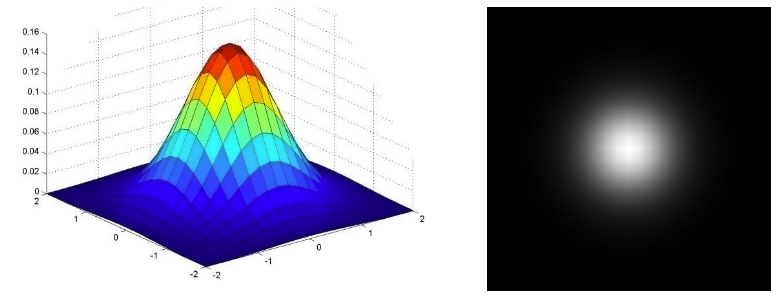
\includegraphics[width=0.9\linewidth]{gaussian_kernel.png}
\end{center}
$$G_\sigma = \frac{1}{2 \pi \sigma^2}^{- \frac{(x^2 + y^2)}{2 \sigma^2}}$$

We can use the Gaussian Kernel for image smoothing, the best part being that the kernel is separable. The actual amount of smoothing depends on $\sigma$ and the window size. \medskip

If we repeatedly apply the Gaussian filter, we produce the scale space of an image.

\subsubsection{High-Pass Filters}

High-pass filters are used to detect areas of the image where a lot is happening (high frequencies). Examples for these are the Laplacian operator $K$ or the high-pass filter $K'$:
$$ K = 
\begin{bmatrix}
    0 & 1 & 0\\
    1 & -1 & 1\\
    0 & 1 & 0
\end{bmatrix}
\qquad
K' =
\begin{bmatrix}
    -1 & -1 & -1\\
    -1 & 8 & -1\\
    -1 & -1 & -1
\end{bmatrix}
$$

High-pass filters can be used to perform image sharpening $I' = I + \alpha |K * I|$.

\section{Image Features}

Image features are about detecting the location of patterns in images, e.g. edge detection or facial landmarks.


\subsection{Template Matching}

Given an template $t$, e.g. template describing an eye, we want to locate an area, in an image $s$, that best fits this template. Alternatively we could also look for areas that match this template by a certain threshold. \medskip

To search for the best match, we try to minimize the mean squared error. This is the same as maximizing the area correlation:
$$r(p, q) = \sum_{x = -\infty}^\infty \sum_{y = -\infty}^\infty s(x,y) \cdot t(x - p, y - q) = s(p,q) * t(-p, -q)$$


\subsection{Edge Detection}

For edge detection we need to calculate the gradient magnitude $M$ and the gradient orientation $\alpha$:
$$M(x,y)=\sqrt{\left(\frac{\delta f}{\delta x}\right)^2+\left(\frac{\delta f}{\delta y}\right)^2}$$ 
$$\quad \alpha (x,y) = \tan^{-1}\left(\frac{\delta f}{\delta y}\middle /\frac{\delta f}{\delta x}\right)$$



We have previously seen kernels that can detect horizontal edges. To expand on this, we differentiate the following kernels:
$$ \text{Prewitt} 
\begin{bmatrix}
    -1 & 0 & 1\\
    -1 & 0 & 1\\
    -1 & 0 & 1
\end{bmatrix}
\qquad
\text{Sobel} 
\begin{bmatrix}
    -1 & 0 & 1\\
    -2 & 0 & 2\\
    -1 & 0 & 1
\end{bmatrix}
$$

We can also transpose these kernels to detect horizontal edges. From the resulting images (horizontal / vertical edges) we take the log sum squared and use different thresholds to achieve the final result.
\begin{center}
	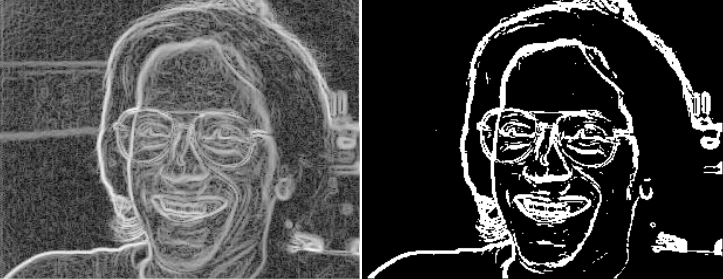
\includegraphics[width=\linewidth]{edge_detection.png}
\end{center}

\subsubsection{Laplacian Operator}

The idea behind the Laplacian operator is to detect discontinuities in the second derivative. This corresponds to detecting zero-crossings. The operator is isotropic (rotationally invariant) and can be implemented with one of the following kernels:
$$
\begin{bmatrix}
    0 & 1 & 0\\
    1 & -4 & 1\\
    0 & 1 & 0
\end{bmatrix}
\quad
\text{ or }
\quad
\begin{bmatrix}
    1 & 1 & 1\\
    1 & -8 & 1\\
    1 & 1 & 1
\end{bmatrix}
$$

This operator is very sensitive to fine details and noise, therefore we might need to blur the image first. Additionally it will respond equally to weak and strong edges, so we want to suppress edges with low gradient magnitude. Blurring and applying the Laplacian operator can be combined into a convolution with Laplacian of Gaussian (LoG). Combining LoG with gradient based threshold delivers the best result.
\begin{center}
	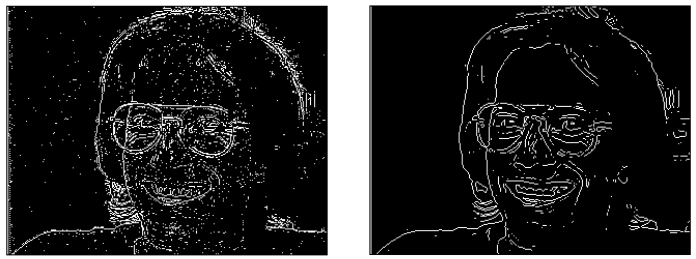
\includegraphics[width=\linewidth]{log_edge_detection.png}
\end{center}

\subsubsection{Canny Edge Detector}

The Canny edge detector works by first smoothing the image with a Gaussian filter. Then we compute the gradient magnitude (Sobel, Prewitt, ...) and the angle of the gradient. After this we want to apply non-maxima suppression to the gradient magnitude image. Combining this with double thresholding, to detect strong and weak edge pixels, and rejecting weak edge pixels not connected with strong edge pixels, results in the Canny edge detector.
\begin{center}
	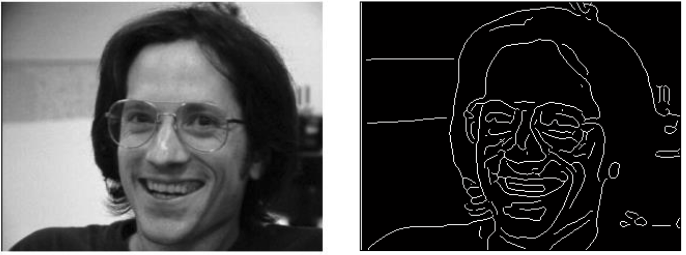
\includegraphics[width=\linewidth]{canny_edge_detection.png}
\end{center}


\subsection{Hough Transform}

Hough transform can be used to find higher order entities in an image, e.g. lines or circles. The Hough transform is a generalized template matching technique. Considering detection of straight lines (y = mx + c), for each edge pixel there are infinitely many possible lines. We plot these possible lines in the 2D space formed by its parameters, we end up with a single line.
\begin{center}
	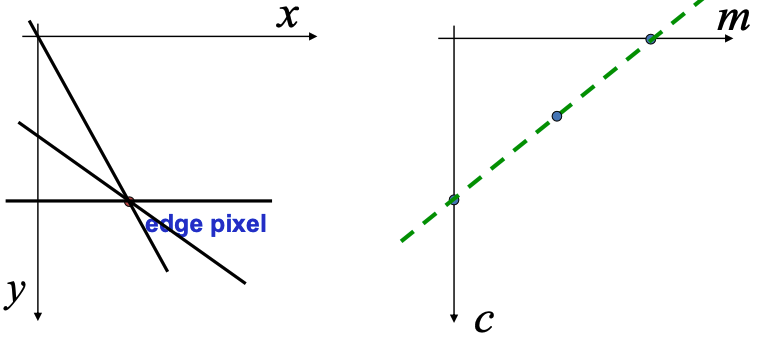
\includegraphics[width=\linewidth]{hough_transform.png}
\end{center}

If we do this for multiple edge points and subdivide the parameter space into discrete bins, we can find the bin with the most possible lines. This gives us the detected line.
\begin{center}
	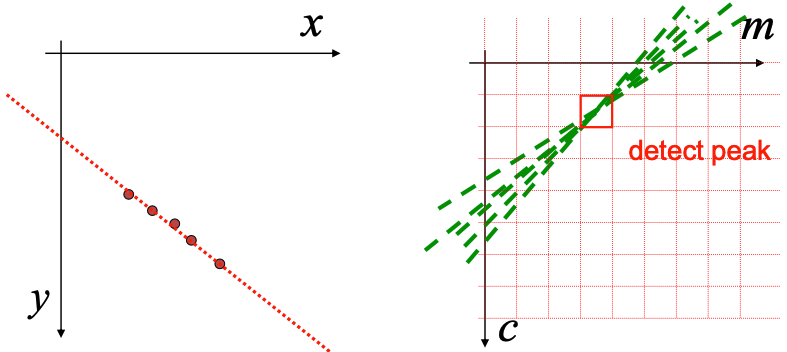
\includegraphics[width=\linewidth]{hough_transform2.png}
\end{center}

There is a problem with this approach, the parameter space is infinite. To avoid this problem we choose an alternative parametrization, in this case we represent a line as an angle and the distance from the origin. Now the representations in parameter space are not lines but sine waves. Again we find the maxima to find our lines.
\begin{center}
	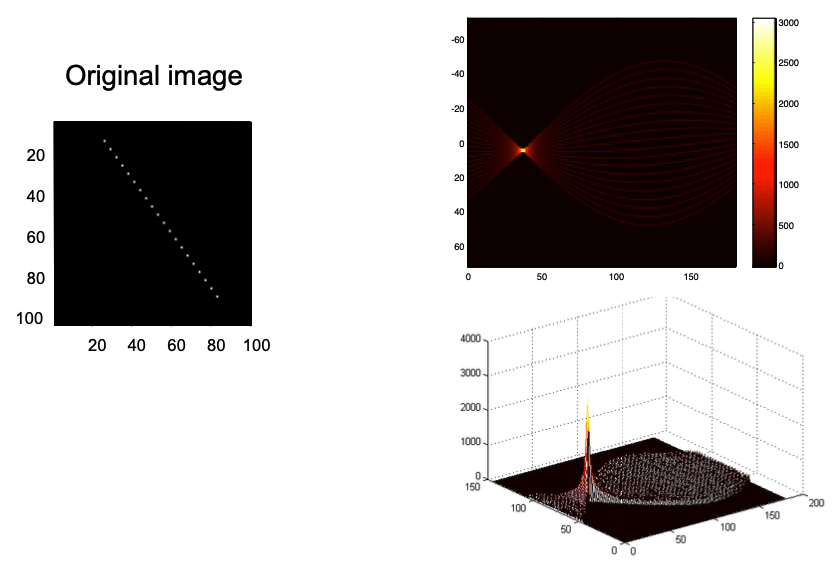
\includegraphics[width=\linewidth]{hough_transform3.png}
\end{center}

To find multiple lines we do non-maxima suppression and keep every strong peek. To expand this concept to circle detection we simply change the parameter space. \medskip

One downside is that two line segments that lie on the same line but are some difference apart cannot be distinguished but appear as a single line.


\subsection{Keypoint Detection}

We might want to only find corners and not edges. We want this corner localization to be accurate, invariant and robust. We define the following:
$$\textbf M = \left( \sum_{(x,y) \in \text{window}} 
\begin{bmatrix}
    f_x^2(x,y) & f_x(x,y) f_y(x,y) \\
    f_x(x,y) f_y(x,y) & f_y^2(x,y)
\end{bmatrix}
\right)$$

$$S(\Delta x, \Delta y) = (\Delta x, \Delta y) \textbf{ M } (\Delta x, \Delta y)^\top$$

Hereby $f_x$ is the horizontal gradient and $f_y$ the vertical gradient. $\textbf{M}$ is called the structure matrix or nomal matrix. To detect feature points we know try to find points for which $\min \Delta^\top \textbf M \Delta, || \Delta || = 1 $ is large. This is the same as maximizing the eigenvalues of $\textbf M$. The eigenvalue allow us to define a measure of "cornerness" (smaller $k$ means more strict):
$$C(x,y) = \det \textbf M - k \cdot (\text{trace } \textbf M)^2 = \lambda_1 \lambda_2 - k \cdot (\lambda_1 + \lambda_2)^2$$

If we plot the values for the eigenvalues, we can divide the space as follows:
\begin{center}
	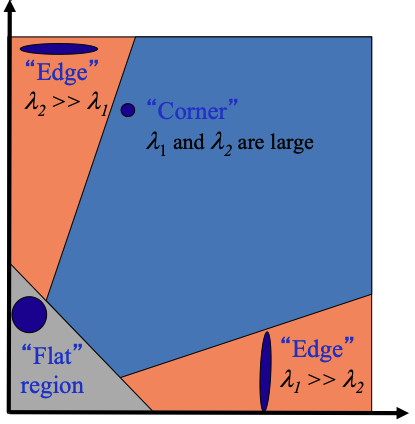
\includegraphics[width=0.6\linewidth]{keypoint_detection.png}
\end{center}

One problem of this approach is that it is not invariant to scale. \medskip

To compare different images, e.g. for combining images. We use thresholded image gradients that are sampled over an array of locations in scale space. This can then be used for example to stich images together (SIFT).







\section{Fourier Transformation}

We have already seen the problem of aliasing. Now we want to understand how we can avoid aliasing and for this we introduce the \textbf{Fourier Transformation}. \medskip

The idea behind the Fourier transformation is to perform a change of basis, where the new basis elements are of the form $e^{-i2\pi (ux + vy)} = \cos (2 \pi (ux + vy)) - i \sin (2 \pi (ux + vy))$ (u, v are the parameters for the new basis).
$$F(g(x,y))(u,v) = \int \int_{R^2} g(x,y) e^{-i2\pi (ux + vy)} dxdy$$

The basis functions of Fourier transform are eigenfunctions of linear systems (one of the reasons it is so popular). Discrete Fourier transformation (DFT) can be represented as:
$$F = \textbf U f$$

Here $\textbf U$ is the Fourier transform base. The vector $(u,v)$ determines the frequency by its magnitude and the orientation by its direction (only looking at the real part):
\begin{center}
	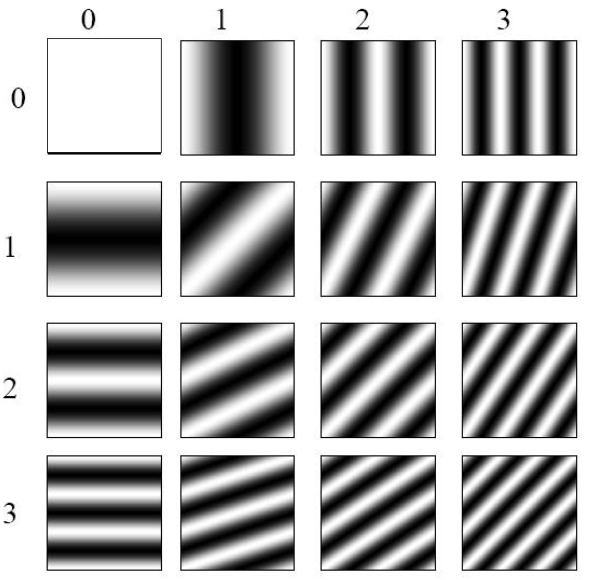
\includegraphics[width=0.6\linewidth]{fourier_transform_pattern.png}
\end{center}


\subsection{Phase and Magnitude}

Since the Fourier transform is complex, it is difficult to plot. Instead we think of the phase (angle) and magnitude (length of the vector) of the transform. Note that natural images have about the same magnitude transform, hence phase seems to matter more. The phase part seems more random than the magnitude. Here you can see an example of the magnitude of an image.
\begin{center}
	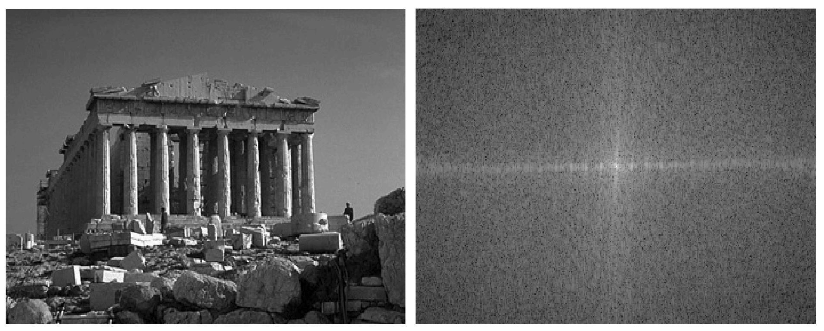
\includegraphics[width=\linewidth]{phase_magnitude.png}
\end{center}


\subsection{Properties of the Fourier Transform}

We already said that the Fourier transform is linear. Further it is important to note that the FT of a Gaussian is a Gaussian. 
\begin{center}
	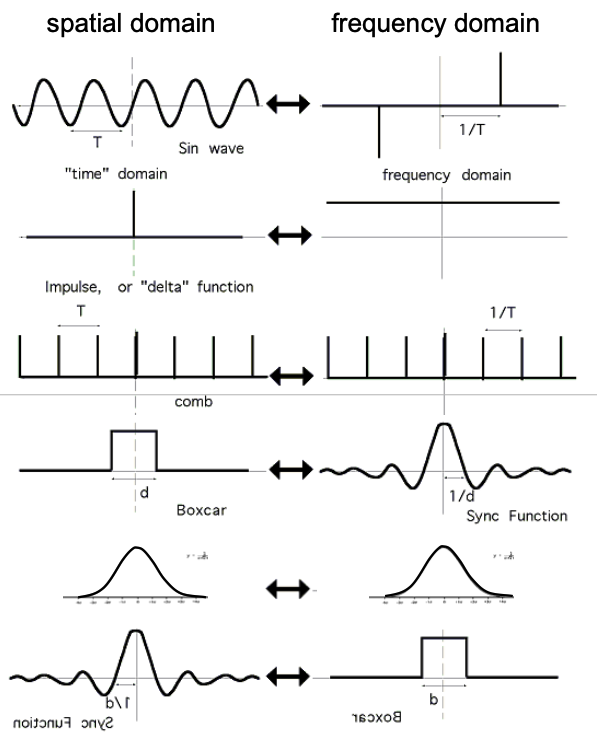
\includegraphics[width=0.7\linewidth]{ft_examples.png}
\end{center}

\textbf{Convolution Theorem} \smallskip

The FT of the convolution of two functions is the product of their FT and the other way around:
$$F \cdot G = \textbf U (f * g), \qquad F * G = \textbf U (f \cdot g)$$


\subsection{Sampling}

Now we have a look at aliasing again. We define our sampling function as follows:
$$\text{Sample}_{2 \text D} (f(x,y)) = f(x,y) \sum_{i = - \infty}^\infty \sum_{j = - \infty}^\infty \delta (x-i, y-j)$$

Where $\delta$ is the Dirac delta function. The FT of a sampled signal now corresponds to:
$$F(\text{Sample}_{2 \text D} (f(x,y)))) = \sum_{i = - \infty}^\infty \sum_{j = - \infty}^\infty F(u-i, v-i)$$

This approach can still lead to aliasing as high frequencies can lead to trouble. To avoid this we first need to suppress high frequencies before sampling. We can do this by convolution with a low-pass filter, this corresponds to multiplying the FT with the same filter. As a low-pass filter we use a Gaussian. \medskip

\textbf{Nyquist Sampling Theorem} \smallskip

To understand why we need to do the low-pass filtering, we can take a look at the Nyquist sampling theorem: \textit{The sampling frequency must be at least twice the highest frequency (of the signal)}.


\subsection{Signal Reconstruction}

In image reconstruction we want to recreate our image from the samples data. To avoid pixelation we look at different reconstruction filters.
\begin{center}
	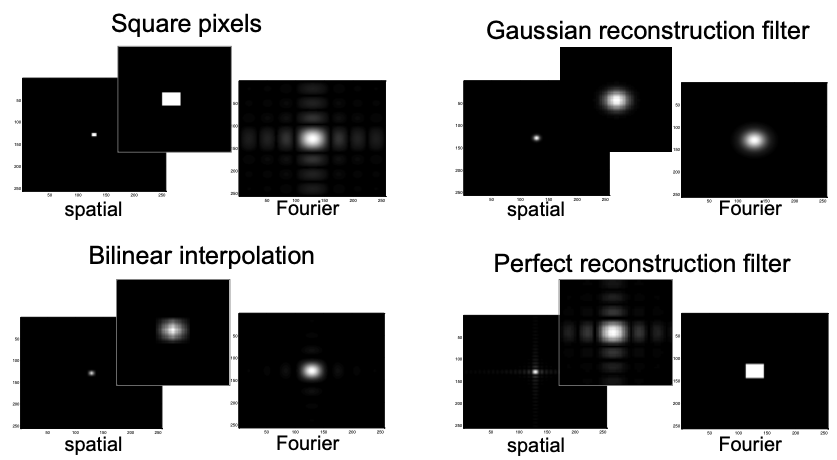
\includegraphics[width=\linewidth]{reconstruction.png}
\end{center}

In the Fourier domain, determining the inverse of a kernel / filter becomes a lot easier, as:
$$F(h)(u,v) \cdot F(h^{-1})(u,v) = 1$$

With this we can for example try to remove motion blur from images. But we have to be careful to regularize our reconstruction filter to avoid noise amplification.

\section{Unitary Transforms}

Images can be either written as matrices or as vectors to make math easier. So a linear image processing system can be defined as:
$$g = \textbf A f$$

So we ask ourself the question how to choose $\textbf A$. We say $\textbf A$ is unitary (or orthonormal for real values) if $\textbf A^{-1} = \textbf A^H$. Transformations by unitary matrices are energy conserving, meaning the length of the transformed vector will stay the same.

We introduce the following notation: $f_i$ one image, $F = [f_1, ..., f_n]$ collection of images and $R_{ff} = E[f_i \cdot f_i^H] = \frac{F \cdot F^H}{n}$ image collection auto-correlation function. While unitary transformations preserve the energy, it will often be unevenly distributed among coefficients. The autocorrelation matrix of the transformed image will look like this: 
$$R_{cc} = \textbf A R_{ff} \textbf A^H$$

The eigenmatrix $\Phi$ of $R_{ff}$ is unitary and defined as follows:
\begin{center}
	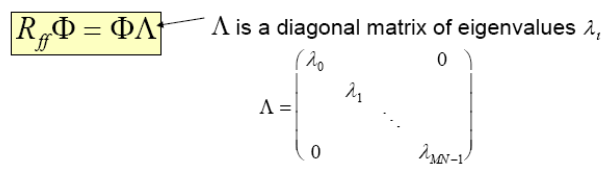
\includegraphics[width=\linewidth]{eigenmatrix.png}
\end{center}

\subsection{Karhunen-Loeve Transform / PCA}

If we choose $\textbf A = \Phi^H$ we get:
$$R_{cc} = \Phi^H R_{ff} \Phi = \Phi^H \Phi \Lambda = \Lambda$$

We can interpret this transformation as follows: "No other unitary transformation packs as much energy into the first $k$ coefficients, where $k$ is arbitrary". The mean squared approximation error by choosing only the first $k$ coefficients is minimized. 
\begin{center}
	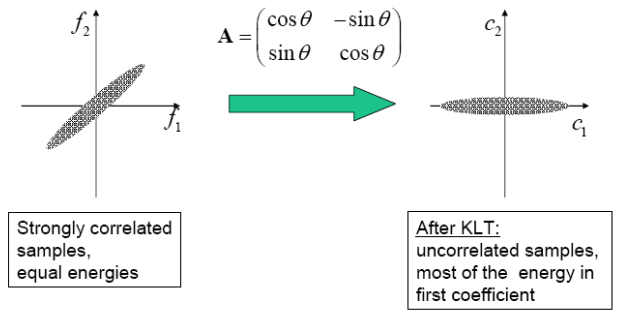
\includegraphics[width=\linewidth]{energy_concentration.png}
\end{center}

The basis images, which are the eigenvectors of the autocorrelation matrix, are called \textbf{eigenimages}. We can use eigenimages for recognition tasks, as the high dimensionality of the images space can be reduced to $k$ dimensions. To perform recogintion, we tailor a KLT / PCA to the specific set of images we want to recognize, for example this lead to Eigenfaces. \medskip

The first principal component is the eigenvector with the largest eigenvalue. The eigenvalue can be interpreted as denoting the variance in the direction of the corresponding eigenvector. So the principal component shows in which direction the data is most spread out.

\subsubsection{Fisherfaces}

To improve on the short comings of Eigenfaces, Fisherfaces try to find the direction where the ratio between individual variance are maximized. As the math behind this is rather complex, it is left out.
\begin{center}
	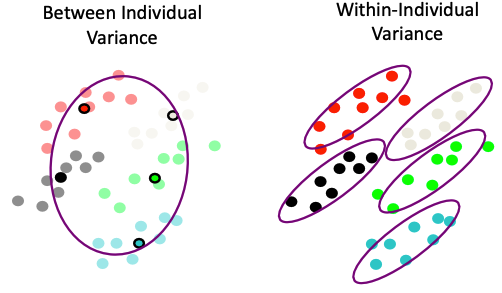
\includegraphics[width=0.8\linewidth]{fisher.png}
\end{center}


\subsection{JPEG Compression}

We notice that humans do not resolve high frequencies too well, therefore we can leave some of them away to reduce the size of an image.
\begin{center}
	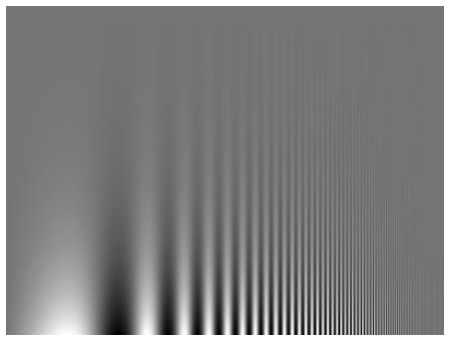
\includegraphics[width=0.8\linewidth]{campbell_robson.png}
\end{center}

This is one of the main concepts in JPEG compression. Instead of FT, JPEG uses discrete cosine transform (DCT), which has no imaginary part. We go through the components of the DCT in a snake like pattern.
\begin{center}
	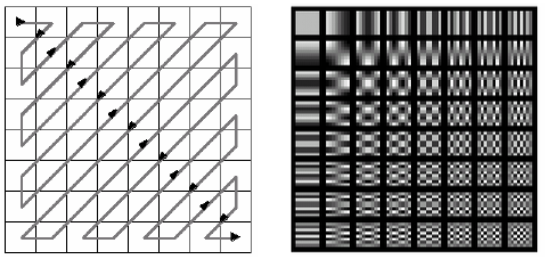
\includegraphics[width=\linewidth]{jpeg_compression.png}
\end{center}

If the coefficients get too small after a certain point, we simply leave them away. In the end we apply Huffman encoding to further reduce the size of our image. \medskip

JPEG tends to introduce three kinds of distortions:
\begin{itemize}
	\item General loss of sharpness and oscillations around high-contrast edges: these are due to approximating intensity transitions with smooth functions (cosines).
	\item Blocking structure: image is processed separately for every 8x8 block, block edges become visible at high compression ratios.
	\item Loss of color detail: the program may aggressively "downsample" chromaticity channels.
\end{itemize}

\section{Pyramids and Wavelets}

The \textbf{scale-space} is the family of signals generated by successive smoothing with a Gaussian filter. Using the scale-space we can downsample the image step by step, giving us an \textbf{image pyramid}.
\begin{center}
	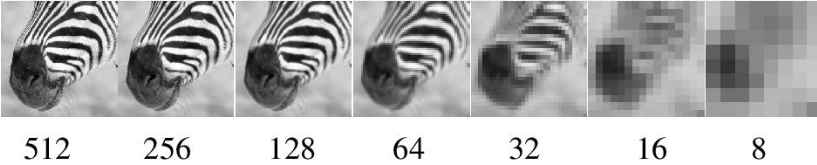
\includegraphics[width=\linewidth]{image_pyramid.png}
\end{center}

Such image pyramids can be used for edge tracking, search for correspondence, etc. One of their main benefits is that they allow for control of detail and computational costs. 


\subsection{The Laplacian Pyramid}

While the Gaussian pyramid successively suppressed high frequencies, the Laplacian pyramid represents a different frequency at each level. This is similar to a bandpass filter.
\begin{center}
	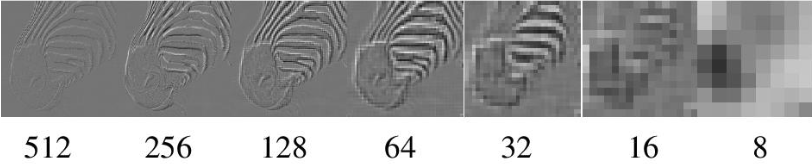
\includegraphics[width=\linewidth]{laplacian_pyramid.png}
\end{center}

With a Laplacian pyramid we mean a difference of Gaussians (DoG). The main benefit is that it removes the redundancy of having the lower frequency parts in every level.


\subsection{Wavelet Transform}

The \textbf{Haar transform} is one of the most basic wavelets.
\begin{center}
	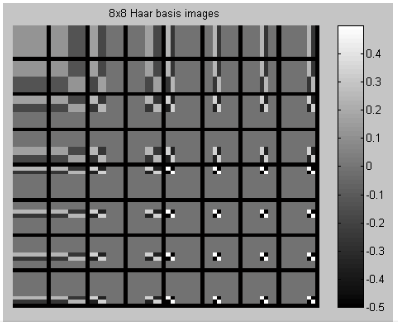
\includegraphics[width=\linewidth]{haar_basis.png}
\end{center}

We can see that the outer vectors correspond to recursively applying a two-band filter to the bands of the previous stage (like a pyramid). The Haar transformation has poor energy compaction, meaning it is not really good for image compression. \medskip

In general wavelet transform works by splitting the signal into a low frequency and a high frequency pass, then the process is applied to the low frequency band recursively.
\begin{center}
	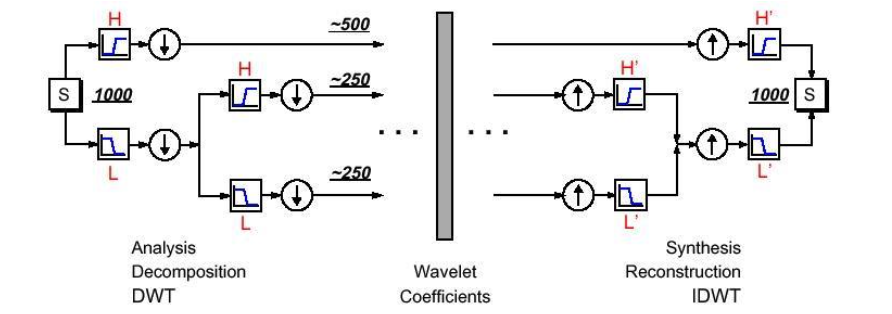
\includegraphics[width=\linewidth]{wavelets.png}
\end{center}

This concept is then again expanded to 2D images.
\section{Optical Flow}

The goal of optical flow is to estimate motion in videos. It is used for tracking, motion segmentation, video stabilization, compression, etc. Optical flow is defined as apparent motion of brightness patterns. This definition is important, as uniform, moving objects have an optical flow of zero, while non moving objects with change in lighting can have an optical flow not equal to zero. \medskip

We define $I(x,y,t)$ as the brightness of at $(x,y)$ at time $t$. So the optical flow constraint is given by the equation:
$$\frac{\mathrm{d} I}{\mathrm{d} t} = \frac{\partial I}{\partial x} \frac{\mathrm{d} x}{\mathrm{d} t} + \frac{\partial I}{\partial y} \frac{\mathrm{d} y}{\mathrm{d} t} + \frac{\partial I}{\partial t} = I_x u + I_y v + I_t = 0$$


\subsection{Aperture Problem}

If we look at the previous equation, we see that we have two unknowns $u$ and $v$, meaning we have an under constraint problem. This is called the \textbf{aperture problem}. The simplest solution to this problem is called the \textbf{normal flow}.
$$u_\bot = - \frac{I_t}{|\nabla I|} \frac{\nabla I}{|\nabla I|}$$


\subsection{Regularization}

Regularization introduces an additional smoothness constraint:
$$e_s = \int \int (u_x^2 + u_y^2) + (v_x^2 + v_y^2) dxdy$$

Beside the optical flow constraint:
$$e_c = \int \int (I_x u + I_y v + I_t)^2 dx dy$$

Now we try to minimize $e_s + \lambda e_c$. This can lead to errors at boundaries as it is the opposite of what we try to enforce with the smoothness term.


\subsection{Lucas-Kanade}

We introduce the assumption of a single velocity for all pixels within an image patch:
$$E(u, v) = \sum_{x, y \in \Omega} \left( I_x(x, y)u + I_y(x, y)v + I_t \right)^2$$

We now have the constraints:
$$\frac{\mathrm d E(u, v)}{\mathrm u} = 0 \qquad \frac{\mathrm d E(u, v)}{\mathrm v} = 0$$

We solve with:
$$
\begin{bmatrix}
	\sum I_x^2 & \sum I_x I_y \\
	\sum I_x I_y & \sum I_y^2
\end{bmatrix}
\begin{pmatrix}
	u \\
	v
\end{pmatrix}
= -
\begin{pmatrix}
	\sum I_x I_t \\
	\sum I_y I_t
\end{pmatrix}
$$

This is equivalent to:
$$\textbf M \textbf U = \left( \sum \nabla I \nabla I^\top \right) \textbf U = - \sum \nabla I I_t = b$$

The Lucas-Kanade algorithm works by computing \textbf U for at each pixel and then solving $\textbf M \textbf U = b$. \textbf M is singular if all gradients point in the same direction, i.e. only normal flow is available. \medskip

We can refine our estimates by repeating the process multiple times.


\subsection{Coarse to Fine}

There are some failure modes to the local gradient method, for one if the intensity structure within our window is poor (uniform area). Another failure mode is when the displacement is too large or the brightness is not constant or if we have no spatial coherence. To make our approach more robust, we can again use an image pyramid, first estimating the optical flow on a coarse image and then iteratively start using finer images from the pyramid.


\subsection{Parametric Motion Models}

Global motion models offer more constraint solutions and integration over larger areas. For affine motions (rotation, translation, sheer) we introduce the following model:
$$I_x (a_1 + a_2 x + a_3 y) + I_y (a_4 + a_5 x + a_6 y) + I_t = 0$$

As each pixel provides one constraint in six global unknowns, we need a minimum of six pixels. The error we try to minimize here is again the square loss. \medskip

We can change the model further to allow for more types of transformation / warping of the image. There are also model that allow for 3D motion.
 
 
\subsection{SSD Tracking}
 
For large displacements we can use template matching, we do this by defining a small area around the pixel as the template and match the next image against that template. This will not work for uniform or noisy patches.
 
\section{Video Compression}

One of the main concepts of video compression is that while the human visual system is specifically sensitive to motion, some distortions are not as perceivable as in static images. Visual perception is limited to $<24$Hz, but flicker can be perceived up to $>60$Hz. \medskip

\textbf{Bloch's Law} \smallskip

Up to a time frame of 100ms, it does not matter "how" light arrives only the sum, e.g. 10ms of double the intensity is equal to 20ms at the normal intensity.


\subsection{Video Format}

A video sequence is a bunch of images aligned in a time sequence. The interlaced video format uses two temporal shifted half images and increases the frequency from $25$Hz to $50$Hz. 
\begin{center}
	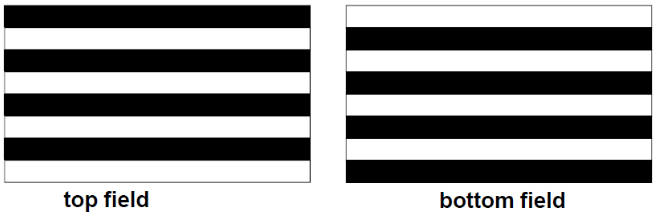
\includegraphics[width=\linewidth]{interlaced.png}
\end{center}

Today this is not done anymore, we rather use a progressive format that updates the whole screen at a time.


\subsection{Temporal Redundancy}

One way of compressing video is to take advantage of similarity between successive frames. Especially for high frame rates this works well. \medskip

The most used representation along the temporal dimension are predictive methods. There we define tree typed of frames:
\begin{itemize}
	\item \textbf{I Frame}: Intra-coded frame, independent of all other frames
	\item \textbf{P Frame}: Predictively-coded frame, based on the previous I and P frame
	\item \textbf{B Frame}: Bi-directionally predicted frame, based on both the previous and future I and P frames
\end{itemize}
\begin{center}
	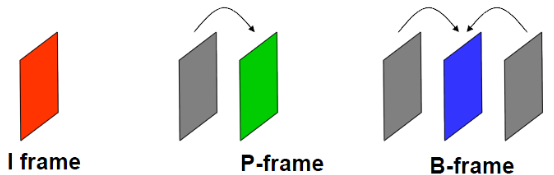
\includegraphics[width=\linewidth]{temporal_frames.png}
\end{center}

P frames can send motion vector plus changes. The frames starting at an I frame until the next I frame is also called a group of pictures (GOP). Temporal redundancy becomes inefficient if there are many scene changes or there is a lot of motion, e.g. \href{https://www.youtube.com/watch?v=r6Rp-uo6HmI&feature=youtu.be}{confetti}.

\subsubsection{Motion-Compensation Prediction}

One possibility of dealing with a high amount of motion is to use MC-prediction. Ideally we would partition the video into moving objects and describe these object motions. In reality this is very difficult, therefore we partition each frame into blocks, e.g. $16$x$16$ pixels, and try to describe the motion of each block.
\begin{center}
	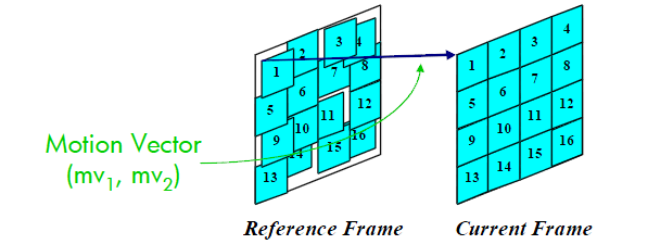
\includegraphics[width=\linewidth]{mc_prediction.png}
\end{center}

The algorithm first divides the frames into blocks and then uses the best matching blocks of the reference frame as prediction of the blocks in the current frame. For the block matching we use some best match metric, e.g. mean squared error or mean average error. The candidate blocks for the best match can either be determined by looking at all blocks or select a subset by some assumptions. \medskip

If we combine all the motion vectors, we end up with a \textbf{motion field} for all the blocks. As motion is not limited to integer-pixel offsets, one could try to estimate sub-pixel motion by spatial interpolation of the frames. The model of MC-prediction does not work well for more complex motions and might produce blocking artifacts.


\subsubsection{Bidirectional MC Prediction}

Instead of only looking at the previous frame we also take a look at the next frame. Bidirectional MC-prediction then estimates the position of a block in the current frame from either the previous frame, the next frame or the average of the previous and next frame.


\subsection{Video Compression Architecture}

Basic video compression architectures use temporal, spatial and color redundancies. Spatial redundancy uses DCT on the blocks and color redundancy does a color space conversion. A basic encoder could look as follows:
\begin{center}
	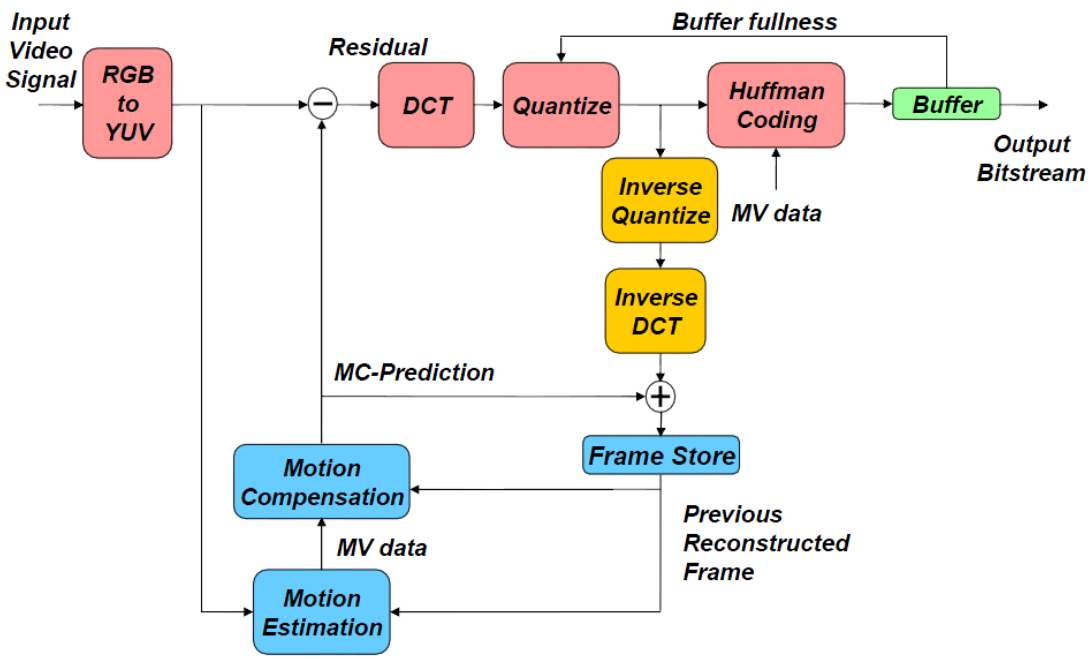
\includegraphics[width=\linewidth]{encoder.png}
\end{center}

The corresponding decoder then looks like this:
\begin{center}
	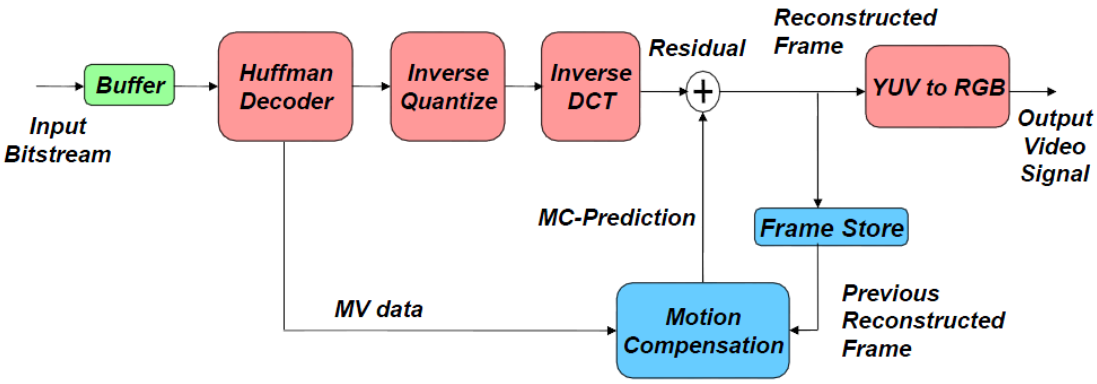
\includegraphics[width=\linewidth]{decoder.png}
\end{center}
\section{Radon Transform}

Radon transformation is often used in medical imaging, e.g. computed tomography (CT). In CT data collection works by shooting x-rays through the material we try to image and collect them on the other side. If we do this from multiple angles, we can try to reconstruct an image from the measured data, as different material absorb a different amount of x-rays. We take the logarithm of this value, since absorption is a multiplicative process. \medskip

This can be seen as an image reconstruction problem.
\begin{center}
	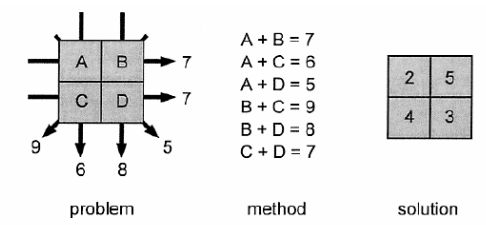
\includegraphics[width=\linewidth]{radon.png}
\end{center}

X-rays move along a straight line, at distance $s$ it has intensity $l(s)$ and after traveling $\delta s$ the intensity is reduced by $\delta l$. The reduction depends on the intensity and the optical density $u(s)$ of the material. For small $\delta s$ it holds $\delta l / l(s) = -u(s) \delta s$. This leads to the following equations:
$$I_{\text{finish}} = I_{\text{start}} \cdot e^R \qquad R = \int_L u(s)ds$$

This related to the Radon transform:
$$Rf(L) = \int_L f(x) |dx|$$

Given the following setup:
\begin{center}
	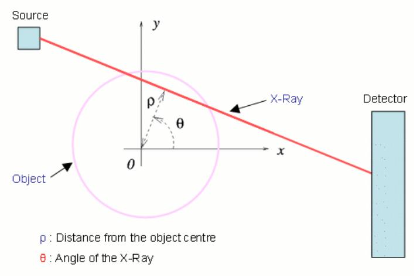
\includegraphics[width=0.8\linewidth]{data_aquisition.png}
\end{center}

We can calculate:
$$R(p, \theta) = \int_{-\infty}^\infty \int_{-\infty}^\infty u(x,y) \delta(p - x \cos \theta - y \sin \theta) dx dy$$

The Radon transform has the following properties:
\begin{itemize}
	\item Linearity
	\item Shifting only changes the $p$ coordinate
	\item Rotation of the coordinate system also rotates the Radon transformation
	\item The Radon transform of a 2D convolution is a 1D convolution of the Radon transformed function with respect to $p$
\end{itemize}

The following image shows the Radon transform of a square. We call this a \textbf{sinogram}.
\begin{center}
	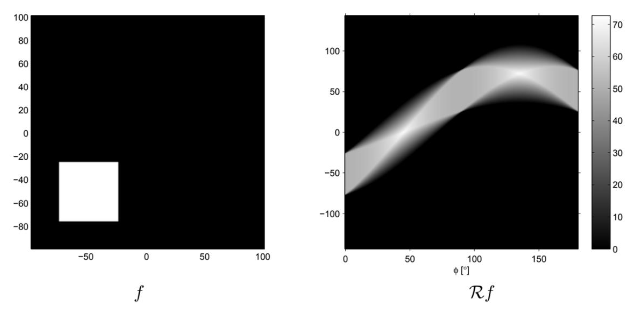
\includegraphics[width=\linewidth]{radon_square.png}
\end{center}


\subsection{Backtransformation}

Up until know we have seen how to perform a Radon transformation from an image to a sinogram. In reality we want the opposite, as medical imaging devices give us a sinogram and we want to reconstruct the image. This is the same as the question: "Can we find $u(x,y)$ if we know $R(p, \theta)$. \medskip

We can compute this with linear algebra, solving the overdetermined system $K f = g$ using normal equations. This solution is not cheap, therefore we are interested in alternative ways. One possible way of doing this would be backprojection:
\begin{center}
	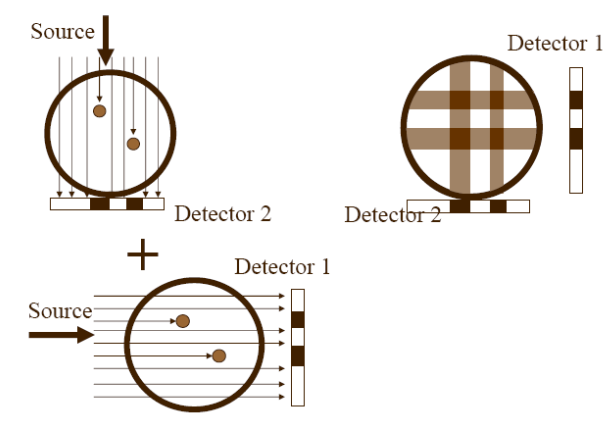
\includegraphics[width=\linewidth]{backprojection.png}
\end{center}

If we do this multiple times, adding more projections, we end up with a blurred version of the original image.

\subsubsection{Fourier / Central Slice Theorem}
$$G(q, 0) = F(q \cos 0, q \sin 0)$$

This tells us that the 1D Fourier transformation of the measurement $g = Rf$ (for a fixed $\theta$) is equal to the 2D Fourier transformation of the object slice $f(x,y)$ evaluated at a particular point. We can apply this for any orientation $\theta$.

\subsubsection{Backprojection Algorithm}
The backprojection algorithm works as follows, for each of the $K$ projection angles $\theta$:
\begin{enumerate}
	\item Measure projection data $P_\theta(t)$
	\item Fourier transform it to find $S_\theta(w)$
	\item Multiply by weighting function $2 \pi |w| / K$ (high-pass filter)
	\item Sum over the image plane and perform 2D inverse Fourier transform.
\end{enumerate}

\begin{center}
	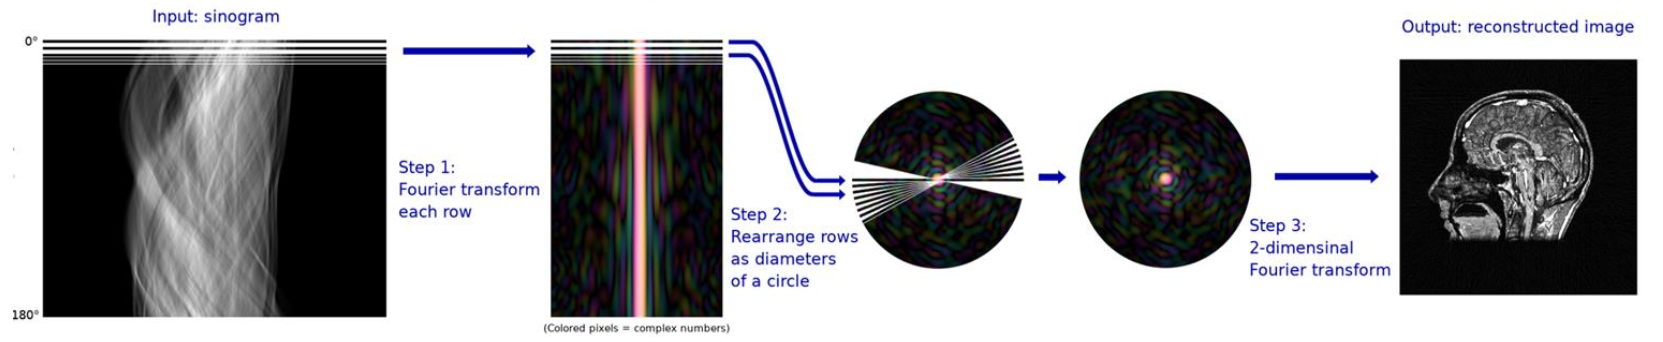
\includegraphics[width=\linewidth]{radon_fourier.png}
\end{center}

There are some practical issues, as it requires many precise measurements and is sensitive to noise it may lead to blurring in the final image.
\section{Sparsity}

We can use sparsity for image restoration. The idea behind this is, that a sparse signal is good for representing structure but not for white Gaussian noise. For this we model an image as follows:
$$\underbrace{y}_{\text{measured image}} = \underbrace{x}_{\text{original image}} + \underbrace{w}_{\text{noise}}$$

Now we perform MAP (maximum a posteriori) estimation:
$$E(x) = \frac{1}{2} ||y-x||_2^2 + \text{Pr}(x)$$

Where Pr is a log prior. Some classical priors to use would be smoothness ($\lambda || \mathcal L x||_2^2$ or total variation $\lambda ||\nabla x ||_1^2$. \medskip

Let $\mathbf D = [d_1, ..., d_p]$ be a set of normalized basis vectors, we call it \textbf{dictonary}. $\mathbf D$ is adapted to $x$ if it can represent it with few basic vectors, meaning a sparse vector $\alpha$ exists, so that $x \approx \mathbf D \alpha$. \medskip

There are predefined dictionaries, but we can also try to learn one ourself. We use the following model:
$$\min_{\alpha} \frac{1}{2} ||x - \mathbf D \alpha||_2^2 + \lambda \psi (\alpha)$$

Here $\psi$ induces sparsity and can be the $l_0, l_1, ...$ norm (we call it Lasso if $l_1$ is used). This idea can be expanded to not only perform denoising, but also do inpainting and demosaicking.


\section{Texture}

The key issues for textures are analysis / segmentation, representing the texture, and synthesis, generating textures.

\subsection{Representing Textures}

Textures are made up of stylised subelements, repeated in meaningful ways. To represent a texture we can try to find these subelements and represent their statistics. Finding the subelements can be done by applying filters and looking at the magnitude of the response. Possible filters could be spots and oriented bars at a variety of different scales (image pyramids).

\subsection{Texture Synthesis}

There is a variety of approaches to texture synthesis. One might use a histogram to capture the intensity probability distribution, but this does not capture any spatial relations. To improve on that one might use a co-occurrence matrix, having the probability distributions for intensity pairs. Other approaches are image-base, trying to perform "cut and paste". This is done by assuming Markov property and computing $P(p | N(p))$ ($N$ is the neighborhood of $p$).
\begin{center}
	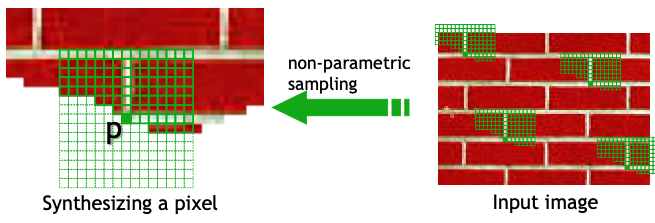
\includegraphics[width=\linewidth]{texture_syntezis.png}
\end{center}

To synthesize $p$, just pick one match at random. This can be expanded to work on patches of images and not single pixels.

\begin{center}
	\Large{\textbf{Computer Graphics}}
\end{center}

\section{Graphics Pipeline}

The graphics pipeline contains all the steps we need to get from a geometric representation to a image. As an input we get not only the geometric representation (e.g. triangle mesh), but also information about materials, lighting and a virtual camera position. \medskip

The pipeline then consists of the following steps:
\begin{enumerate}
	\item \textbf{Modeling Transform} - Take the object and transforms it into world coordinate space
	\item \textbf{Viewing Transform} - Transforms the world coordinate space into camera coordinate space
	\item \textbf{Primitive Processing} - Transforms the geometric representation into a triangle mesh
	\item \textbf{3D Clipping} - Removes triangles not visible to the camera (objects outside the frustum)
	\item \textbf{Projection to Screen Space} - Projects from 3D camera space to 2D screen space
	\item \textbf{Scan Conversion} - Converts triangles to pixels and interpolates attributes
	\item \textbf{Lighting, Shading, Texturing} - Computes color based lighting, shading and texture map
	\item \textbf{Occlusion Handling} - Updates the color buffer using the depth buffer (z-buffer), deal with objects that are hidden by other objects
	\item \textbf{Display} - Output to the display
\end{enumerate}

If we perform the lighting, shading, texturing step after the scan conversion, we call it \textbf{pixel shading}, if it is the other way around, we call it \textbf{vertex shading}. \medskip

\textbf{Programmer's View} \smallskip

From a programmers point of view the graphic pipeline looks as follows:
\begin{center}
	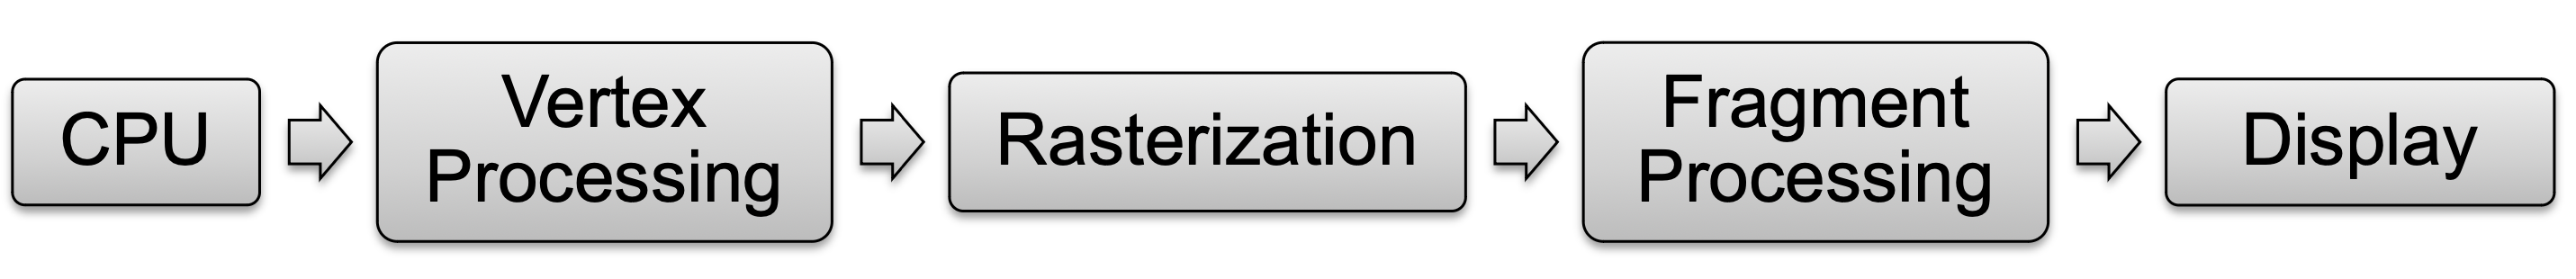
\includegraphics[width=\linewidth]{programmer_view.png}
\end{center}

Vertex processing deals with per-vertex operations (vertex shaders) and fragment processing deal with per-pixel operations (fragment shaders).

\section{Light and Colors}

To understand colors in computer graphics, we first have to learn about the real physical properties of colors.


\subsection{What is light?}

Light is a form of electromagnetic radiation, we perceive a very limited section of the spectrum as visible light.
\begin{center}
	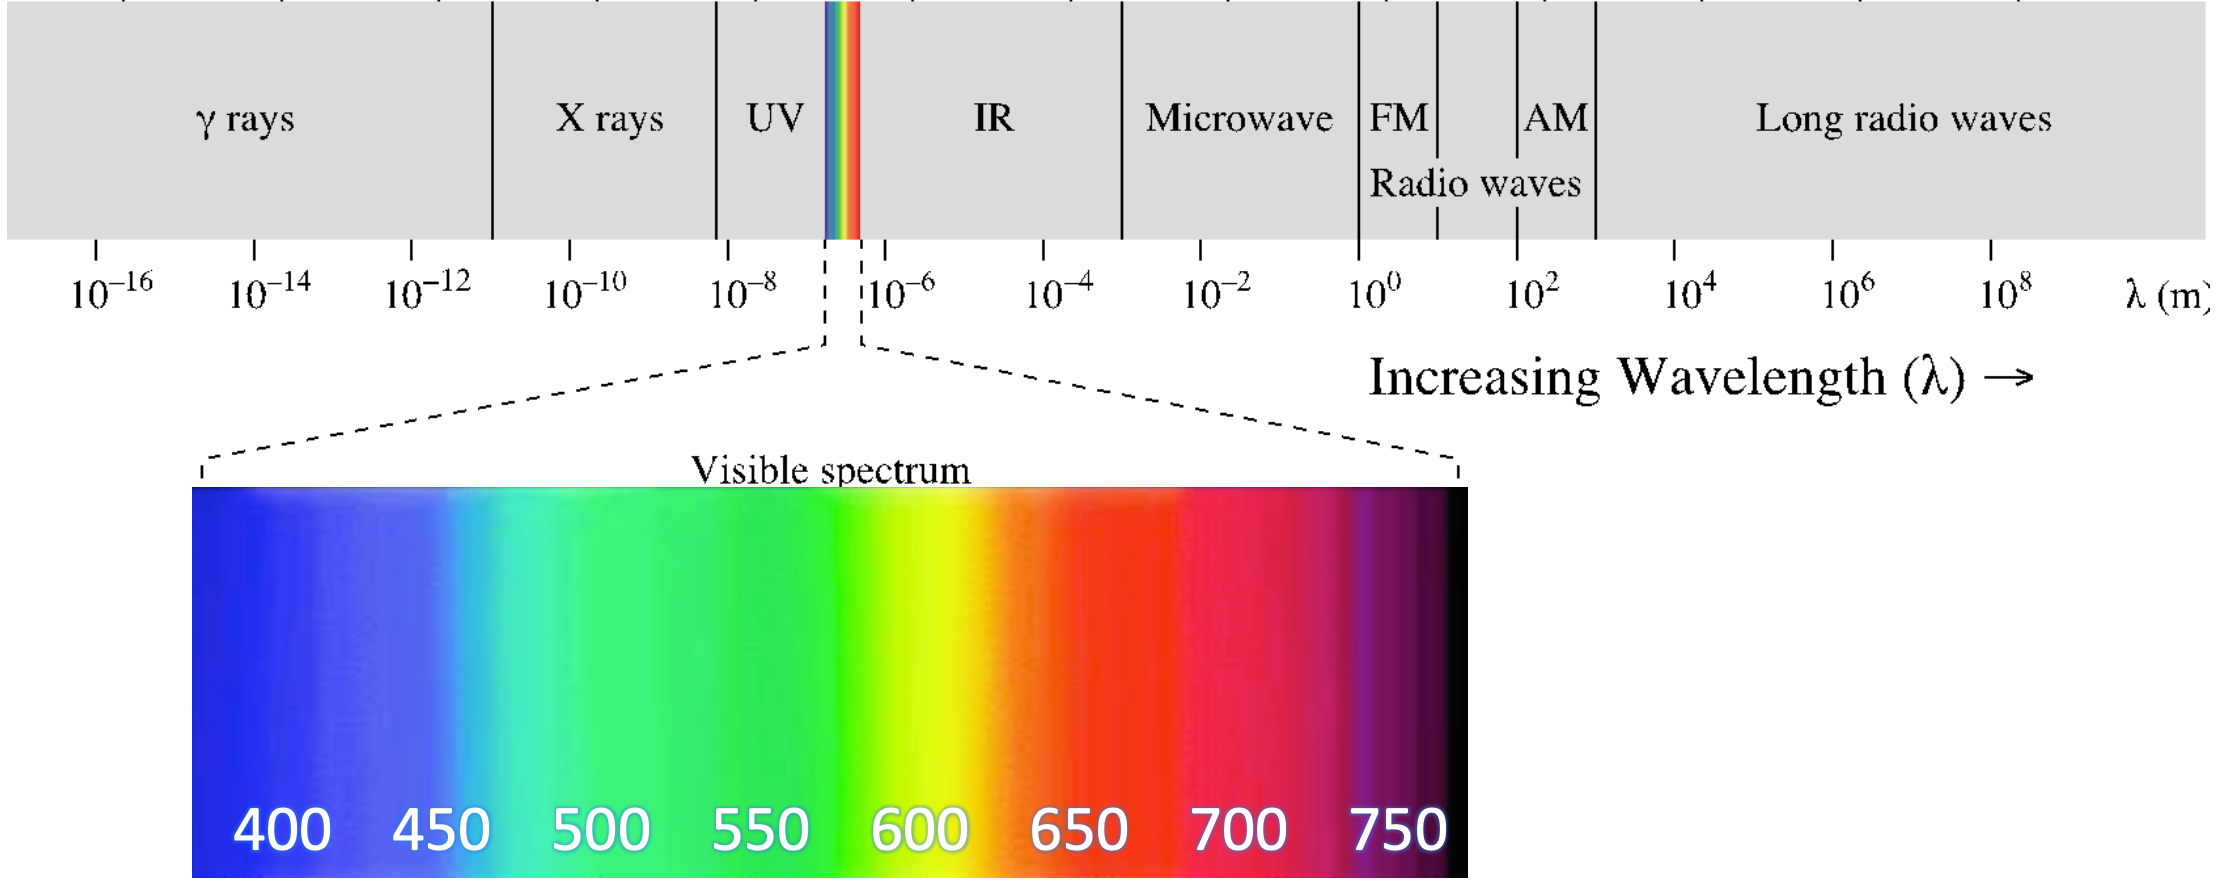
\includegraphics[width=\linewidth]{light_spectrum.png}
\end{center}

Light can be a mixture of many wavelength and is typically defined by the spectral power distribution (SPD). $P(\lambda)$ defines the intensity of this spectrum at wavelength $\lambda$. We humans then perceive this distribution as colors. A light ray carries more information than a human can process, so we project this spectrum onto a 3D subspace given by the types of cones.


\subsection{Anatomy of the Eye}  

On our retina there are two types of different cells, rods and cones. While rods respond to intensity only, the cones respond to color. There are three type of cones, each responding to a different wavelength (short = blue, medium = green, long = red). These cones are the reason we project the infinite dimensional space $P(\lambda)$ onto a 3D subspace.


\subsection{Defining the Subspace}

When doing this projection we will inherently lose some information, therefore two different SPD might look the same to us. There have been multiple attempts to standardise this subspace and the projection used. \medskip

\textbf{The CIE Primary System} \smallskip

This was one of the the first attempts at standardising the color subspace. Their approach was to try to define every color by an additive mixture of the three base colors red, green, blue. They came up with the following results:
\begin{center}
	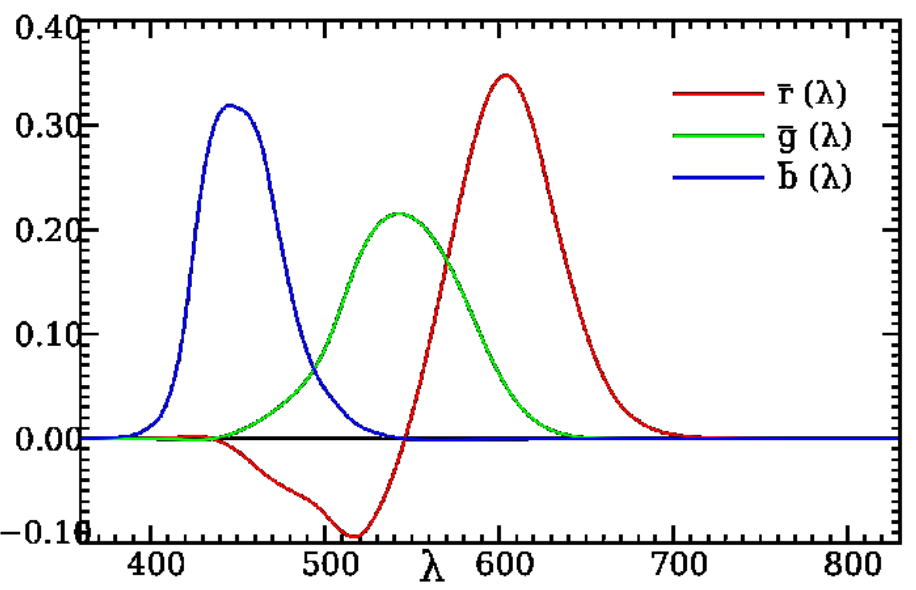
\includegraphics[width=0.8\linewidth]{rgb_mixture.png}
\end{center}

This shows that there are some colors that cannot be reproduced (negative r value). The CIE XYZ color space defines transformation from these three curves to a vector $(X, Y, Z)$. 
$$X = \int_0^\infty P(\lambda) \bar x (\lambda) d\lambda$$
$$Y = \int_0^\infty P(\lambda) \bar y (\lambda) d\lambda$$
$$Z = \int_0^\infty P(\lambda) \bar z (\lambda) d\lambda$$

The transformation matrix from RGB to XYZ is then given by:
$$\begin{pmatrix}
	\bar x(\lambda) \\
	\bar y(\lambda) \\
	\bar z(\lambda) \\
\end{pmatrix}
=
\begin{pmatrix}
	2.36 & -0.515 & 0.005 \\
	-0.89 & 1.426 & 0.014 \\
	-0.46 & 0.088 & 1.009 \\
\end{pmatrix}
\begin{pmatrix}
	\bar r(\lambda) \\
	\bar g(\lambda) \\
	\bar b(\lambda) \\
\end{pmatrix}
$$

These transformed curves have the properties that they are normalized, positive definite and the $\bar y (\lambda)$ curve corresponds to the luminance.

\begin{center}
	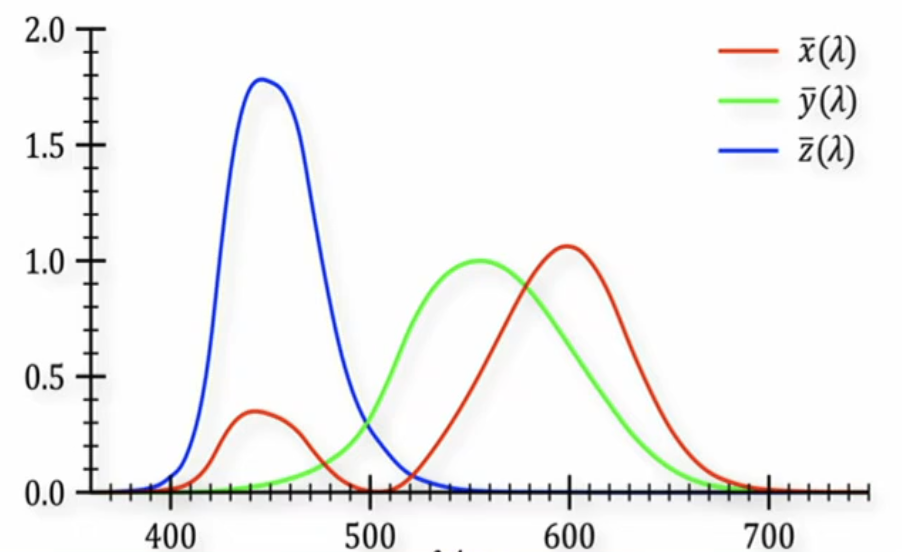
\includegraphics[width=0.8\linewidth]{XYZ.png}
\end{center}

As the XYZ color space is 3D, it is often not very practical. Therefore we normalize the XYZ components and project it into a 2D space:
$$x = \frac{X}{X + Y + Z} \qquad y = \frac{Y}{X + Y + Z}$$

To reverse is given by:
$$X = x \cdot \frac{Y}{y} \qquad Z = \frac{Y}{y} - x \cdot \frac{Y}{y} - Y$$

Now $(x,y)$ characterize color and $Y$ characterizes brightness. If we plot $(x,y)$ on a plane, we get all the colors of a single brightness (chromaticity chart).
\begin{center}
	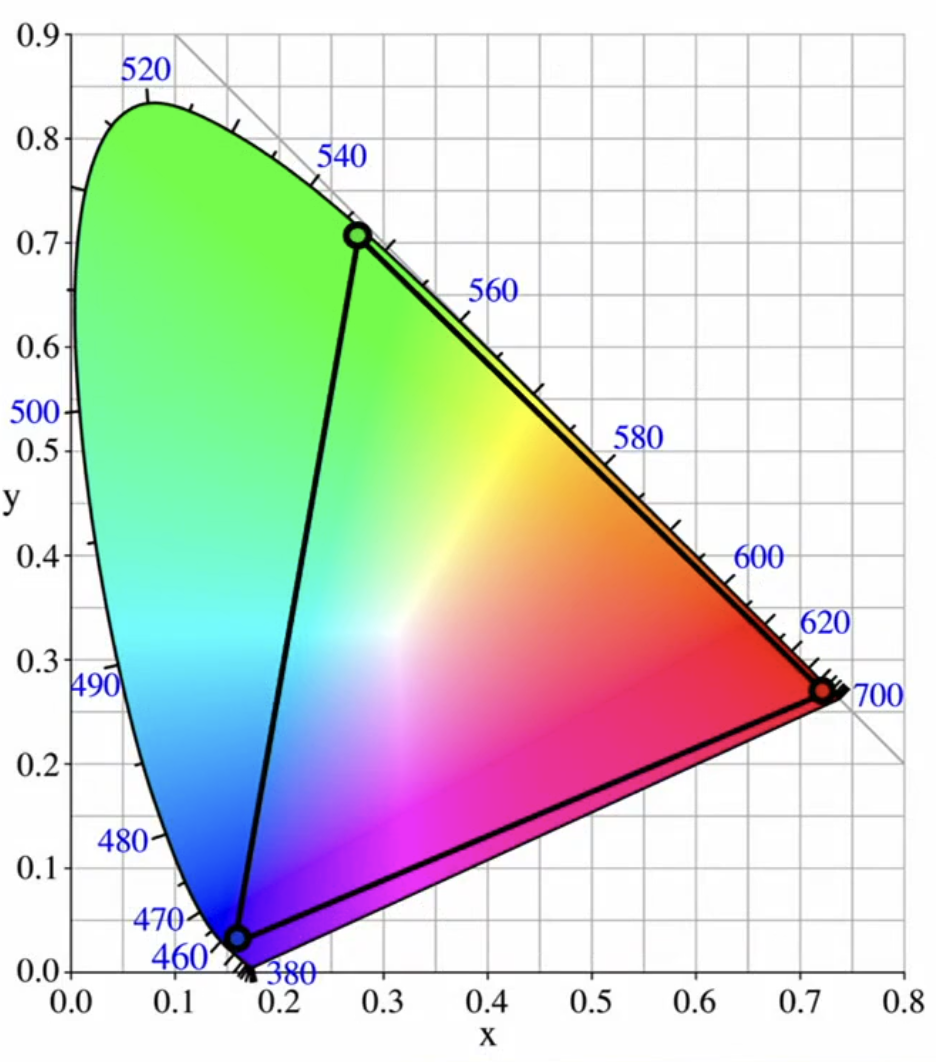
\includegraphics[width=0.65\linewidth]{horseshoe.png}
\end{center}
 
The primary colors are on the boundary of the horse shoe and all linear combinations of two colors are on a line. Screens are limited to a combination of three colors (triangle  in the chart), so they can not show all possible colors.\medskip

\textbf{Other Color Spaces}\smallskip

The \textbf{CMY color space} is the inverse of the RGB space.
$$\begin{pmatrix}
	C \\ M \\ Y
\end{pmatrix} = \begin{pmatrix}
	1 \\ 1 \\ 1
\end{pmatrix} - \begin{pmatrix}
	R \\ G \\ B
\end{pmatrix}$$

The \textbf{HSV color space} consists of hue (base color), saturation (purity of color) and value (brighness). This is a more user oriented color space, as it is rather intuitive to interact with. \medskip

\textbf{MacAdams} ellipses describe an area around a color, such that everything inside the ellipse is perceptual indistinguishable.
\begin{center}
	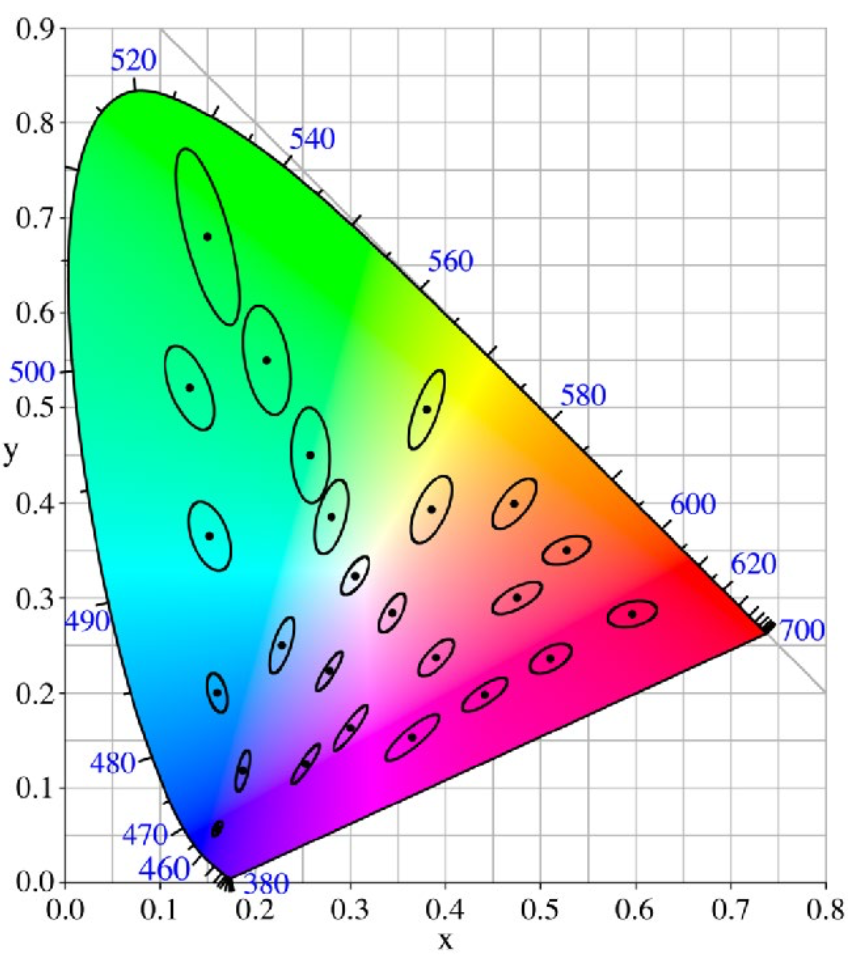
\includegraphics[width=0.5\linewidth]{macadams.png}
\end{center}

The \textbf{CIELAB and CIELUV color spaces} use MacAdams ellipses and transform the color space, so that the ellipses become nearly circular.
\begin{center}
	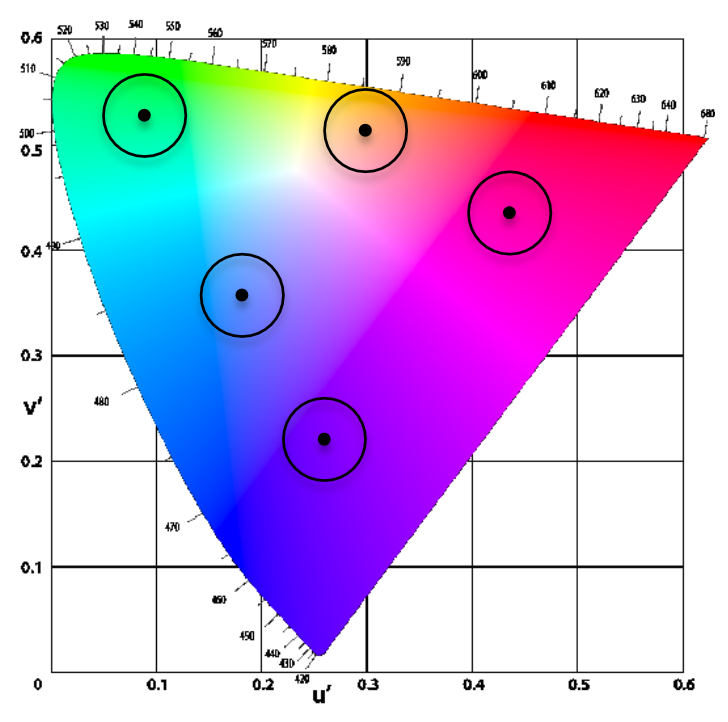
\includegraphics[width=0.5\linewidth]{cieluv.png}
\end{center}


\section{Transformations}

Transformations map geometry. In the graphics pipeline this is mostly used for changing positions and orientations for objects, projecting them to the screen and animating objects.

\subsection{2D Transformations}
\begin{itemize}
	\item Translation - note that translation is not linear as it corresponds to vector addition
	$$\begin{pmatrix}
		x' \\ y'
	\end{pmatrix} = \begin{pmatrix}
		x \\ y
	\end{pmatrix} + \begin{pmatrix}
		t_x \\ t_y
	\end{pmatrix}$$
	
	\item Scaling
	$$\begin{pmatrix}
		x' \\ y'
	\end{pmatrix} = \begin{bmatrix}
		s_x & 0 \\ 0 & s_y
	\end{bmatrix} \cdot \begin{pmatrix}
		x \\ y
	\end{pmatrix}$$
	
	\item Rotation
	$$\begin{pmatrix}
		x' \\ y'
	\end{pmatrix} = \begin{bmatrix}
		\cos \theta & - \sin \theta \\ \sin \theta & \cos \theta
	\end{bmatrix} \cdot \begin{pmatrix}
		x \\ y
	\end{pmatrix}$$
\end{itemize}

Affine maps are linear in homogeneous coordinates (adding one dimension). This allows us to perform translations as a linear operation ($p' = \textbf T p$).

\begin{itemize}
	\item Translation	
	$$\textbf T = \begin{bmatrix}
		1 & 0 & t_x \\ 0 & 1 & t_y \\ 0 & 0 & 1
	\end{bmatrix}$$
	
	\item Scaling
	$$\textbf S = \begin{bmatrix}
		s_x & 0  & 0\\ 0 & s_y & 0 \\ 0 & 0 & 1
	\end{bmatrix}$$
	
	\item Rotation
	$$\textbf R = \begin{bmatrix}
		\cos \theta & - \sin \theta & 0 \\ \sin \theta & \cos \theta & 0 \\ 0 & 0 & 1
	\end{bmatrix}$$
	
	\item Shear along $x$-axis ($a$) and along the $y$-axis ($b$)
	$$\textbf{SH} = \begin{bmatrix}
		1 & a  & 0\\ 0 & 1 & 0 \\ 0 & 0 & 1
	\end{bmatrix} \qquad \textbf{SH} = \begin{bmatrix}
		1 & 0  & 0\\ b & 1 & 0 \\ 0 & 0 & 1
	\end{bmatrix}$$
\end{itemize}

When transforming back from the homogeneous coordinates it is important to divide by the last value. We can easily combine multiple transformation by taking the matrix product.


\subsection{3D Transformations}

We also want to use homogeneous coordinates in the 3D space. 
\begin{itemize}
	\item Translation	
	$$\textbf T = \begin{bmatrix}
		1 & 0 & 0 & t_x \\ 0 & 1 & 0 & t_y \\ 0 & 0 & 1 & t_z \\ 0 & 0 & 0 & 1
	\end{bmatrix}$$
	
	\item Scaling
	$$\textbf S = \begin{bmatrix}
		s_x & 0 & 0 & 0 \\ 0 & s_y & 0 & 0 \\ 0 & 0 & s_z & 0 \\ 0 & 0 & 0 & 1
	\end{bmatrix}$$
	
	\item Rotation - this is \textbf{not commutative} anymore!
	$$\textbf R_x = \begin{bmatrix}
		1 & 0 & 0 & 0 \\ 0 & \cos \theta & - \sin \theta & 0 \\ 0 & \sin \theta & \cos \theta & 0 \\ 0 & 0 & 0 & 1
	\end{bmatrix}$$
	$$\textbf R_y = \begin{bmatrix}
		\cos \theta & 0 & \sin \theta & 0 \\ 0 & 1 & 0 & 0 \\ -\sin \theta & 0 & \cos \theta & 0 \\ 0 & 0 & 0 & 1
	\end{bmatrix}$$
	
	$$\textbf R_z = \begin{bmatrix}
		\cos \theta & - \sin \theta & 0 & 0 \\ \sin \theta & \cos \theta & 0 & 0 \\ 0 & 0 & 1 & 0 \\ 0 & 0 & 0 & 1
	\end{bmatrix}$$
	
	\item Shear parallel to the principal planes
	$$\textbf{SH}_{xy} = \begin{bmatrix}
		1 & 0 & sh_x & 0\\ 0 & 1 & sh_y & 0 \\ 0 & 0 & 1 & 0 \\ 0 & 0 & 0 & 1
	\end{bmatrix}$$
	$$\textbf{SH}_{xz} = \begin{bmatrix}
		1 & sh_x & 0 & 0\\ 0 & 1 & 0 & 0 \\ 0 & sh_z & 1 & 0 \\ 0 & 0 & 0 & 1
	\end{bmatrix}$$
	
	$$\textbf{SH}_{yz} = \begin{bmatrix}
		1 & 0 & 0 & 0\\ sh_y & 1 & 0 & 0 \\ sh_z & 0 & 1 & 0 \\ 0 & 0 & 0 & 1
	\end{bmatrix}$$
\end{itemize}


\subsection{Coordinate Systems}

A coordinate system represents a point / vector as a linear combination of orthonormal basis vectors.
$$p = p_x x + p_y y + p_z z$$

A change of coordinate systems consists of a combination of translation and rotation:
$$p' = \textbf T \textbf R p = \begin{bmatrix}
	r_1 & r_2 & r_3 & t \\
	0 & 0 & 0 & 1
\end{bmatrix} \begin{pmatrix}
	p_x \\ p_y \\ p_z \\ 1
\end{pmatrix}$$

We are also interested in how the surface normal $n$ is transformed. Given a transformation $p' = \textbf M p$ the surface normal is transformed by $n' = (\textbf M'{-1})^\top n$.


\subsection{Projection}

When we want to go from 3D space to 2D space, e.g. when projecting to screen space, we have to think about perspective. We differentiate two types of projection.
\begin{center}
	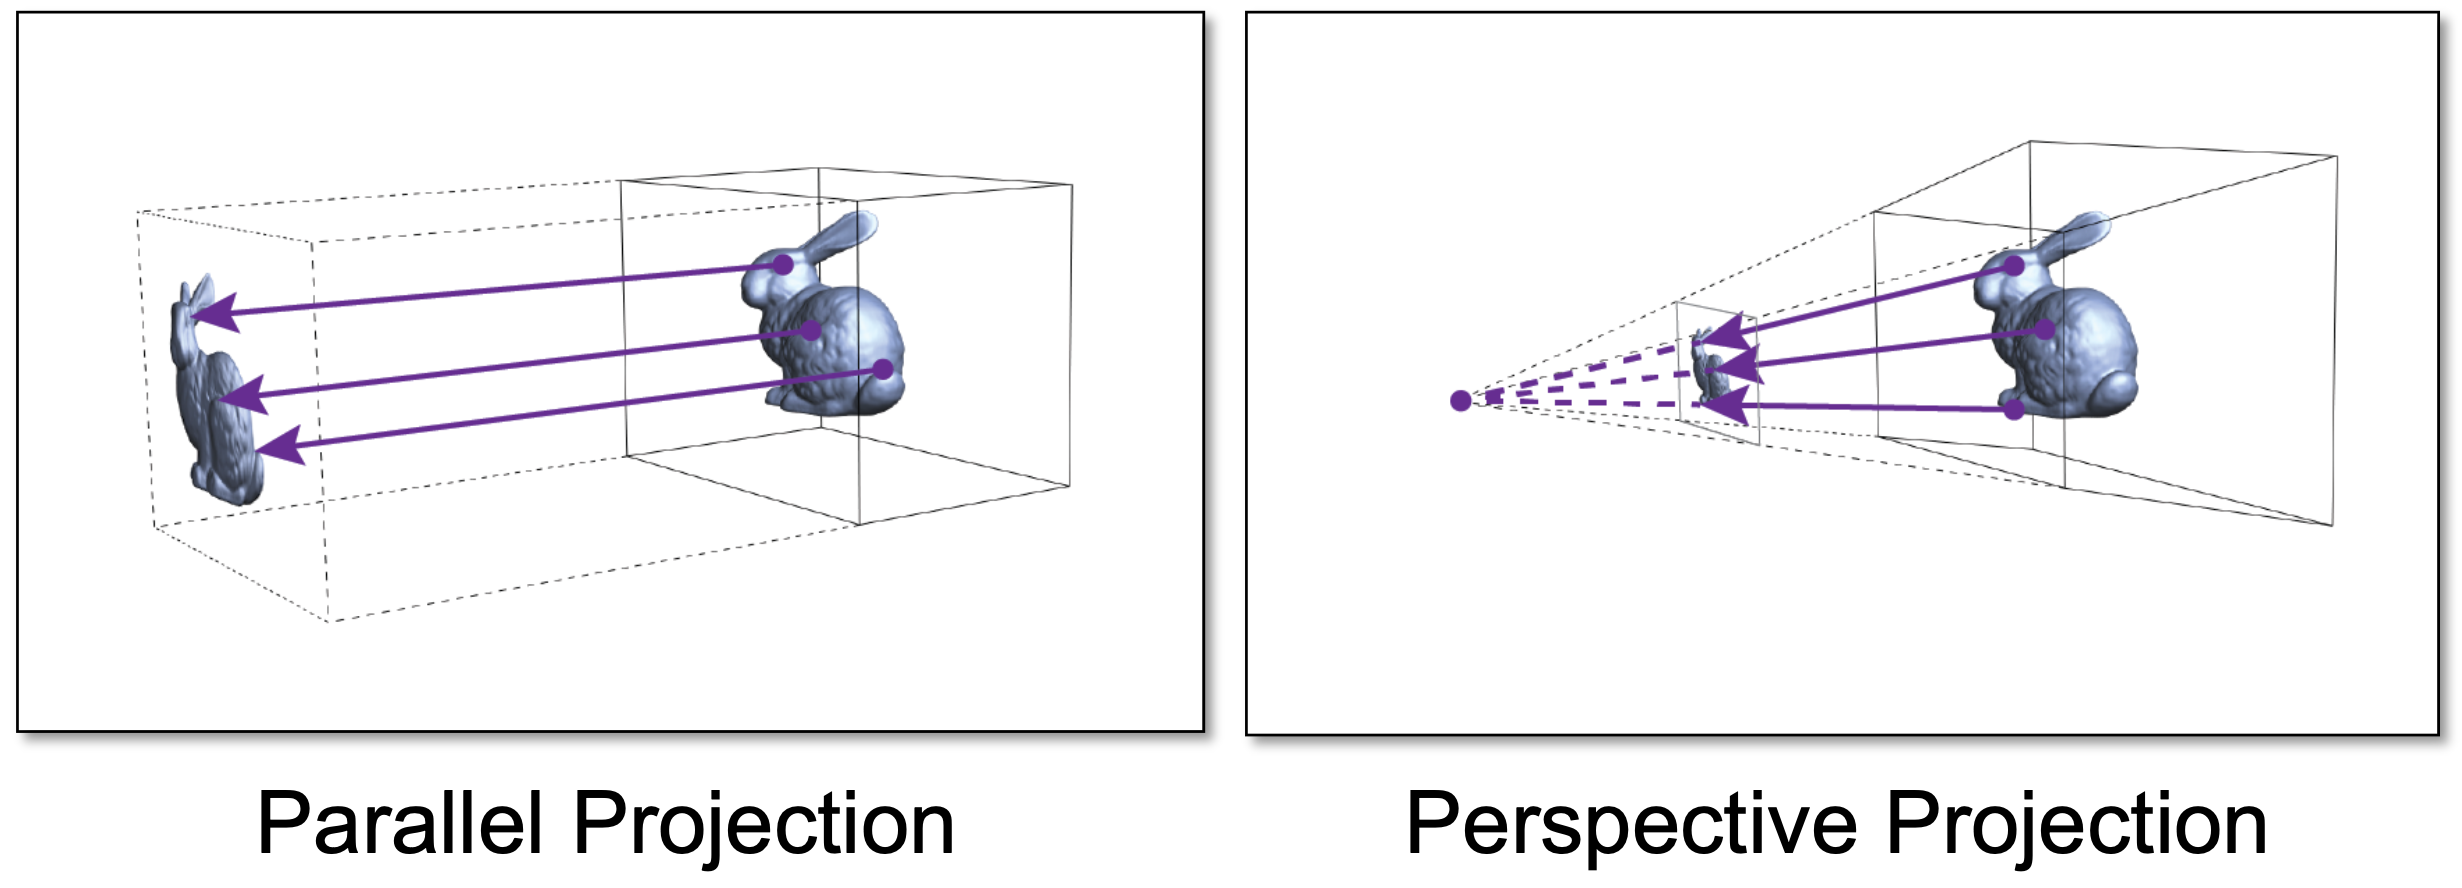
\includegraphics[width=\linewidth]{projection.png}
\end{center}

Perspective projection corresponds to how a camera would see an object. In perspective projection the lines seem to converge in some point, these points are called vanishing points. If we have more than three vanishing points we have multiple center of projection.

\subsubsection{Mathematics of Perspective Projection}

If the camera plane is defined by the $x$ and $y$ axis, i.e. the coordinate system is aligned with the $z$ axis, the math behind the projection is easy. This is the reason we first transform from world coordinates to camera coordinates. For a given focal distance $d$, the projection is then given by:
$$\textbf M p = \begin{bmatrix}
	1 & 0 & 0 & 0 \\
	0 & 1 & 0 & 0 \\
	0 & 0 & 1 & 0 \\
	0 & 0 & 1/d & 0
\end{bmatrix} \begin{pmatrix}
	x \\ y \\ z \\ 1
\end{pmatrix} = \begin{pmatrix}
	x \\ y \\ z \\ z / d
\end{pmatrix}$$

If we transform this back to non homogeneous space, we end up with:
$$\begin{pmatrix}
	dx / z \\ dy / z \\ d
\end{pmatrix}$$

\subsubsection{Mathematics of Parallel Projection}

This is a lot simpler and corresponds to:
$$\textbf M = \begin{bmatrix}
	1 & 0 & 0 & 0 \\
	0 & 1 & 0 & 0 \\
	0 & 0 & 0 & 0 \\
	0 & 0 & 0 & 1
\end{bmatrix}$$




\section{Lighting and Shading}

In lighting we have to differentiate between local and global illumination models. Local illumination models only consider the direct interaction of a light source with an object surface, the global illumination model also considers indirect lighting. We mostly focus on local illumination models.


\subsection{Measuring Light}

Radiometry is the study of measuring electromagnetic radiation, including visible light. We first introduce some definitions:
\begin{itemize}
	\item \textbf{Angle} - $\theta = \frac{l}{r}$, for a circle $2 \pi$ radians
	\item \textbf{Solid Angle} - $\Omega = \frac{A}{r^2}$, for a sphere $4 \pi$ steradians
	\item \textbf{Direction} - point on the unit sphere parameterized by two angles $\omega = (\theta, \phi)$ (zenith and azimuth)
\end{itemize}

\begin{center}
	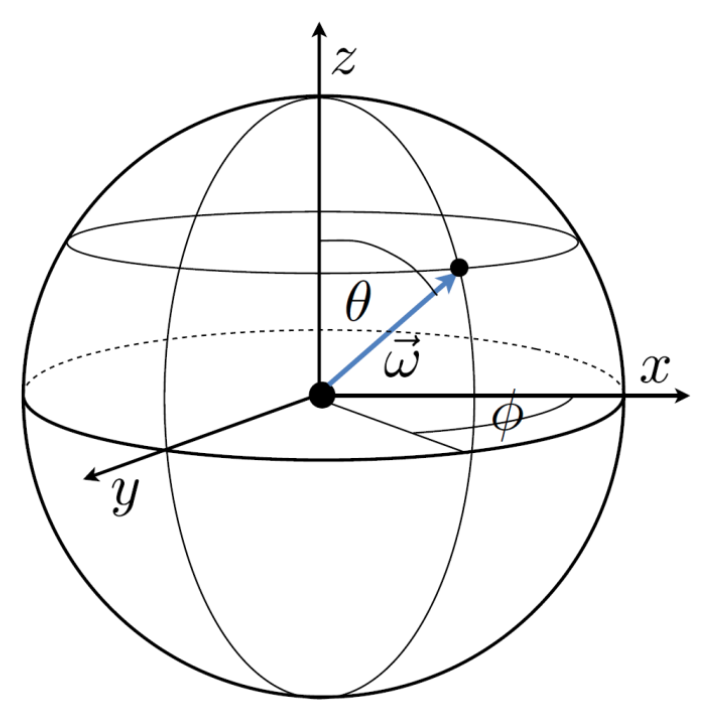
\includegraphics[width=0.5\linewidth]{unit_sphere.png}
\end{center}

Now we can define light as consisting of photons with a position $x$, a direction $\omega$ and a wavelength $\lambda$. Each photon has an energy of $hc / \lambda$. \medskip

The basic quantities to measure light are then defines as:
\begin{itemize}
	\item \textbf{Flux} $\Phi$ - total amount of energy passing through a surface or space per time unit
	\item \textbf{Irradiance} $E$ - flux per unit area arriving at a surface 
	\item \textbf{Radiosity} $B$ - flux per unit area leaving a surface 
	\item \textbf{Intensity} $I$ - flux per solid angle 
	\item \textbf{Radiance} $L$ - intensity per unit area or flux density per unit solid angle 
\end{itemize}
\begin{center}
	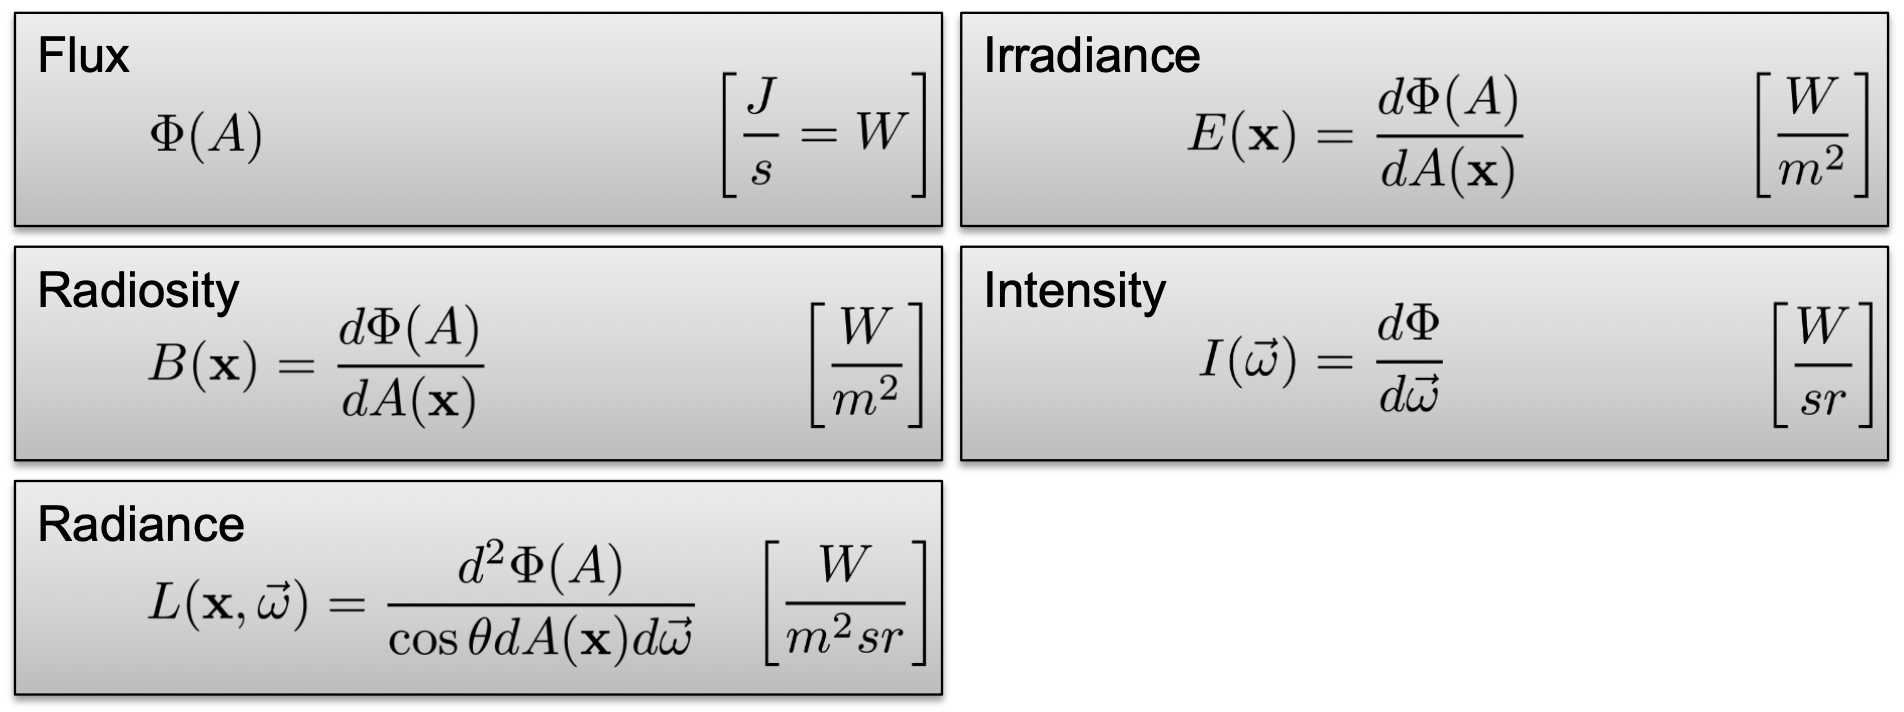
\includegraphics[width=\linewidth]{radiometry.png}
\end{center}


\subsection{Reflection Models}

\subsubsection{BRDF}

Bidirectional Reflectance Distribution Function (BRDF) models the surface and its reflection of light. The BRDF provides a relation between incident radiance and differential reflected radiance.
$$f_r(x, \omega_i, \omega_r) = \frac{dL_r(x, \omega_r)}{L_i(x, \omega_i) \cos \theta_i d \omega_i}$$

From this we can derive the \textbf{reflection equation}:
$$L_r(x, \omega_r) = \int_{H^2} f_r(x, \omega_i, \omega_r) L_i(x, \omega_i) \cos \theta_i d \omega_i$$

The reflection equation describes a local illumination model. BRDF has the ability to express a large variety of complex materials. There are large libraries of measured BRDFs for different materials.

\subsubsection{Simpler Reflections}

These physical based models where for a long time to complex, so a simpler model was used. A material was characterized by a combination of diffuse and specular reflexion.
\begin{center}
	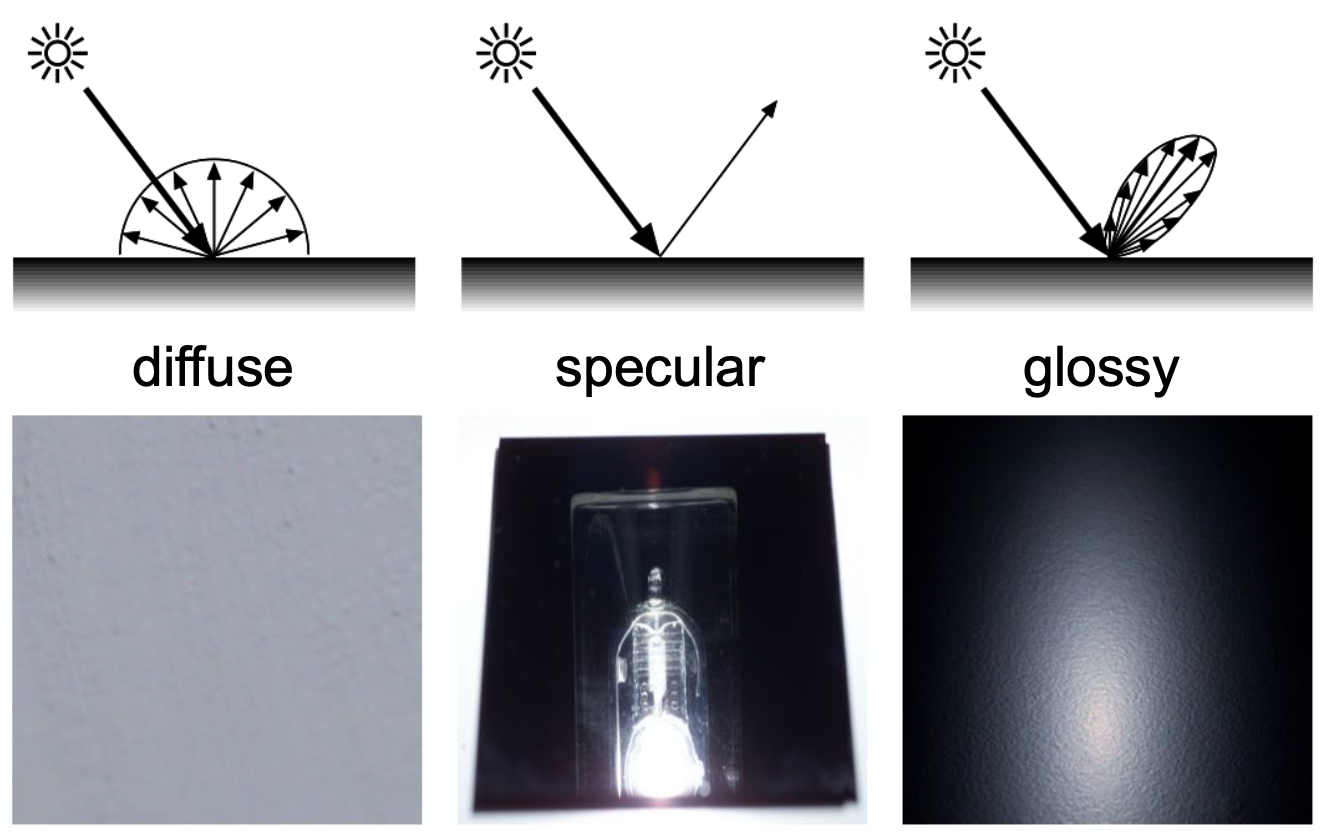
\includegraphics[width=\linewidth]{reflections.png}
\end{center}

For diffuse reflection, the BRDF is a constant, since it is the same value over the whole hemisphere.
$$L_r(x) = f_r E_i(x)$$

\subsubsection{Phong Illumination}

OpenGL uses simplified reflections, one of the most used models is the phong illumination model. \medskip

\textbf{Ambient Light} comes from all directions. Its reflection is independent of the cameras position, light position and surface orientation. So we can model the reflection intensity by using a light source and a material parameter.
$$I = I_a k_a$$

\textbf{Diffuse Reflection} is dependent on directed light $I_p$ (light source position) and the orientation of the source. It still is independent of the camera position. So we can model the reflection intensity by either using a cosine or the dot product using the surface normal.
$$I = I_p k_d \cos \theta = I_p k_d (N \cdot L)$$

In a very simple model, we can now simply take the sum of the ambient light and the diffuse reflection. 
$$I = I_a k_a + I_p k_d (N \cdot L)$$

To improve on this we can add quadratic attenuation due to spatial radiation (quadratically less energy when moving away from the source).
$$I = I_a k_a + f_{att} I_p k_d (N \cdot L) \qquad f_{att} = \frac{1}{d_L^2}$$

To further improve we can add the specular reflection. This depends on the angle between the reflection $R$ and viewing ray $V$.
\begin{center}
	\includegraphics[width=0.7\linewidth]{specular_reflection.png}
\end{center}

Combining this we end up with a simple but already quite good model for lighting.
\begin{center}
	\includegraphics[width=\linewidth]{lighting_model.png}
\end{center}

The phong illumination model approximates specular reflection by cosine powers. It also makes the whole function dependent on the wavelength.
$$I_\lambda = I_{a \lambda} k_a O_{d \lambda} + f_{att} I_{p \lambda} [k_d O_{d \lambda}(N \cdot L) + k_s (R \cdot V)^n]$$


\subsection{Shading Models}

We have seen how to calculate the lighting of an object, now we want to know how to calculate the color per primitive. The simplest model would be to have a single color per primitive, this is called flat shading and happens in screen space. This does not look good as a primitive converts to many pixels.

\subsubsection{Gouraud Shading}

Similar to flat shading, gouraud shading also happens in screen space. It works by calculating the face normals and then the vertex normals by averaging the face normals. After that we evaluate illumination for each vertex and then interpolate the vertex colors bilinearly on the current scan line.
\begin{center}
	\includegraphics[width=0.7\linewidth]{gouraud_scanline.png}
\end{center}

There are a few problems with scan line interpolation. The first one being perspective distortion, as we interpolate in the projection plane. Further the interpolation is orientation dependent and quality depends on the size of primitives.

\subsection{Phong Shading}

Phong shading happens in object space. It works by barycentric interpolation of the surface normals. The color is then determined by the interpolated normal.
\begin{center}
	\includegraphics[width=0.7\linewidth]{phong_interpolation.png}
\end{center}

Phong shading cannot be applied if the normal is not defined.

\subsection{Transparency}

The typical color format includes an alpha channel, indicating the level of transparency. If we have partially transparent object, we need to blend the colors of the different objects together. One approach for this is \textbf{alpha blending}.
\begin{center}
	\includegraphics[width=\linewidth]{alpha_blending.png}
\end{center}

The intensity of the opaque object gets filtered by the object in front of it.
$$I_\lambda = I_{\lambda_1} \alpha_1 \Delta t + I_{\lambda_2} e^{- \alpha_1 \Delta t} \approx I_{\lambda_1} \alpha_1 + I_{\lambda_2} (1- \alpha_1)$$

To evaluate the alpha blending, we need to have an order to the primitives. This is the reason that we store the distance even in the screen space representation. Having that distance value (z-buffering) allows us to apply \textbf{back to front rendering} of the primitives. However this does not work anymore if we have intersecting objects. \medskip

To solve this problem we use \textbf{depth peeling}. It works by using multiple passes, each pass renders the next closest fragment.




















\section{Geometry and Textures}

Geometry plays a fundamental role in CG. At the start, we need to define how we want to represent geometry in a discrete setting. Source data can be acquired by 3D scanning, digital modelling, procedural modelling, etc. We mainly differentiate by data generated on a computer (mesh) vs. data acquired from real-world object (point cloud).


\subsection{Geometry Representation}
 
If we look at geometry representation, we need to think about storage, acquisition / creating of shapes, editing of shapes and rendering of shapes. \medskip

\textbf{Parametric Surfaces} are surfaces that are defined by a parameter space. This allows us to simplify the storage to the position in the parameter space. On the downside, if there is no parameterisation of a surface, this does not work. \medskip

\textbf{Subdivision Surfaces} are surfaces that are piecewise linear. By increasing the subdivision, we can increase the number of surfaces and the precision. \medskip

\textbf{Point Set Surfaces} are a collection of points that can be combined to surfaces. \medskip

\textbf{Polygonal Meshes} store the boundary of objects and the connectivity.
\begin{center}
	\includegraphics[width=0.9\linewidth]{mesh.png}
\end{center}

Todays GPU pipelines are optimized for such mesh structures and therefore provide fast rendering. On a mathematical level we define a polygon by a set of vertices $V = \{v_0, ..., v_{n-1}\}$ and a set of edges $E = \{(v_0, v_1), ..., (v_{n-2}, v_{n-1})\}$. A polygon is planar and non-self-intersecting. \medskip

A polygonal mesh is a set of connected polygons $M = (V, E, F)$ where $F$ are the faces of the polygons. It has the following properties:
\begin{itemize}
	\item Every edge belongs to at least one polygon
	\item The intersection of two polygons in $M$ is either empty, a vertex, or and edge
\end{itemize}

A manifold is a surface locally homeomorphic to a disk.
\begin{center}
	\includegraphics[width=\linewidth]{manifold.png}
\end{center}

In a manifold mesh there are some structures that are not allowed:
\begin{center}
	\includegraphics[width=\linewidth]{non_manifold.png}
\end{center}

Real-world data is often non-manifold.


\subsection{Mesh Data Structures}

We want to store the geometry and topology of a polygonal mesh. This data structure should allow for easy rendering, support geometry queries and allow for modifications. \medskip

\textbf{Triangle Lists} are a simple data structure. On the downside, they do not provide information about connectivity and are largely redundant (vertex gets saved multiple times).
\begin{center}
	\includegraphics[width=0.65\linewidth]{triangle_list.png}
\end{center}

\textbf{Indexed Face Set} are a lot more efficient, store connectivity and eliminate the redundancy. On the other hand geometric queries and modifications are costly.
\begin{center}
	\includegraphics[width=\linewidth]{indexed_face_set.png}
\end{center}


\subsection{Texture Mapping}

On fundamental way to enhance the quality of our renderings are texture mapping. Texture mappings increase the level of detail, without increasing our geometric mesh.
\begin{center}
	\includegraphics[width=\linewidth]{texture_map.png}
\end{center}

The difficulty is to find this mapping (2D to 3D space), this can lead to aliasing, blur or level-of-detail issues. \medskip

Texture mapping creates a one-to-one mapping between the texture and the geometry, this is done by parameterization of our geometric surface. We want the mapping to have the following properties:
\begin{itemize}
	\item Low Distortion
	\item Bijective Mapping
	\item Efficient to Compute
\end{itemize}

Finding a good texture map can be done by using a texture atlas or by finding cuts to transform our 3D surface into 2D. 


\subsection{Texture Filtering}

When we project our texture to a surface it is subject to aliasing.
\begin{center}
	\includegraphics[width=\linewidth]{texture_filtering.png}
\end{center}

Low-pass filtering can help us avoid this aliasing. A typical low-pass filter would be the Gaussian filter. \medskip

Filtering in texture space is different form filtering in screen space. If we have an isotropic Gaussian in screen space this can relate to an anisotropic Gaussian in texture space.
\begin{center}
	\includegraphics[width=0.9\linewidth]{filtering.png}
\end{center}


\subsection{Light Map}

Light maps are a trick to simulate the effect of a local light source.
\begin{center}
	\includegraphics[width=\linewidth]{light_map.png}
\end{center}


\subsection{Environment Map}

Environmental maps are used to render reflective objects efficiently. It works by by intersecting the reflected ray with the surrounding sphere or cube map.
\begin{center}
	\includegraphics[width=\linewidth]{environment_map.png}
\end{center}


\subsection{Bump Mapping}

Bump maps are used to perturb surface normal according to textures, allowing us to represent small-scale geometry (e.g. pores).
\begin{center}
	\includegraphics[width=\linewidth]{bump_map.png}
\end{center}

One limitation of bump mapping is that it does not work on the silhouette.


\subsection{Procedural Textures}

Combining Perlin noise (or other types of noise) in different resolutions, allows us to create procedural textures. One examples for such a texture would be wood textures.

\begin{center}
	\includegraphics[width=\linewidth]{perlin_noise.png}
\end{center}

\section{Processing Signals}

This section focused on topic already covered in the first part of the lecture. Therefore I left out most of the content and only focused on the new content.


\subsection{Antialiasing Filters}

We already used Gaussian filters for antialiasing. A Gaussian Filter is a infinite response filter. The downside to this type of filter is that it is unstable. We mentioned that a Sinc Filter would be even better (ideal low-pass filter), but it is extremely hard to implement. B-Splines are another type of filter we really like, as they are easy to implement and allow for locally adaptive smoothing.


\subsection{Perspective Projection}

Equally distributed samples in texture space can get unequally distributed when projected into screen space. The optimal filter is spatially variant. \medskip

There are two type of problems that happen when projecting. \textbf{Magnification} happens when the pixel in the texture image maps to an area larger than one pixel. To avoid this we can simply use bilinear interpolation. \textbf{Minification} is the oposite, pixels in the texture image map to areas smaller than one pixel. To deal with this problem we use mipmapping. \medskip

\textbf{Mipmapping} is the process of storing the texture at multiple resolutions (image pyramid) and choosing the resolution level depending on the projected size of the triangle.


\subsection{Geometric Aliasing}

This is another problem that happens at the edges of polygons. Since we our screen space allows for only a limited number of pixels, we end up with a staircase pattern for the edges. To lessen this effect we can apply \textbf{supersampling}. \medskip

Supersampling introduces multiple color samples per pixel, which then are averaged. There are multiple possible sampling patterns, including uniform, jittering, stochastic and poisson. The following shows supersampling using jittering.
\begin{center}
	\includegraphics[width=\linewidth]{supersampling.png}
\end{center}

\section{Bezier Curves}


\section{B-Splines}
\section{Subdivision Surfaces}

Subdivision surfaces are a generalization of spline curves / surfaces. They allow for successive refinement and converge to a smooth surface.
\begin{center}
	\includegraphics[width=\linewidth]{subdivision.png}
\end{center}

It relies on corner cutting:
\begin{enumerate}
	\item Insert two new vertices at 1/4 and 3/4 of each edge
	\item Remove the old vertices
	\item Connect the new vertices
\end{enumerate}
\begin{center}
	\includegraphics[width=\linewidth]{corner_cutting.png}
\end{center}

There are multiple algorithms for subdivision, with different properties (applied on polygonal mesh or triangle mesh, $G^1$ or $G^2$ continuous etc.). \medskip

One of these algorithms is the \textbf{Loop Subdivision}. It is a generalization of box splines and can be used on triangle meshes. It generates a $G^2$ continuous limit surface:
\begin{center}
	\includegraphics[width=\linewidth]{loop_subdivision.png}
\end{center}

\section{Scan Conversion}

Scan conversion (also called rasterization) is the problem of converting our objects to the discrete pixel space, e.g. deciding which pixel lie inside our object. 


\subsection{Scan Conversion of Lines}

\textbf{Bresenham lines} choose the closest pixel at each intersection. The goal is to have a fast decision which pixel has to be drawn next. It does this by using the position of the midpoint $m$ with respect to the intersection point $q$ as a criterion.
\begin{center}
	\includegraphics[width=0.7\linewidth]{bresenham.png}
\end{center}

Given $f(x,y) = ax + by + c = 0$ as the implicit equation of the straight line, it decides based on $d = f(m)$. If $d < 0$ select pixel E, else select pixel NE. After the first decision, we can base our update criterion based on the choice E or NE.
$$\text{Pixel NE : } d_{new} = d_{old} + \Delta y - \Delta x$$
$$\text{Pixel E : } d_{new} = d_{old} + \Delta y$$

\subsection{Scan Conversion of Polygons}

Filled polygons (especially triangles) are the most important graphics primitives. The straightforward solution would be to perform an inside test for each pixel, but this is very inefficient. Instead we process scan line after scan line. We call a group of picked pixels inside a scan line a \textbf{span}. The algorithm then works as follows:
\begin{enumerate}
	\item Calculate all intersections of the scan line
	\item Sort the intersection points by ascending x-coordinates
	\item Fill all spans in between two consecutive intersection points if the parity is odd
\end{enumerate}

\begin{center}
	\includegraphics[width=0.9\linewidth]{scan_line.png}
\end{center}
\section{Visibility and Shadows}


\subsection{Visibility}

We already encountered the \textbf{visibility problem}, some parts of some surfaces could be occluded. There are two possible solutions:
\begin{itemize}
	\item \textbf{Painter's Algorithm} - Render objects / polygons from furthest to nearest. This leads to problems when there are intersections or cyclic overlaps.
	\item \textbf{Z-Buffering} - Store depth to the nearest object for each pixel.
\end{itemize}

The Z-Buffering algorithm works as follows:
\begin{enumerate}
	\item Initialize all $z$ values to $\infty$.
	\item For each polygon: If $z$ value of a pixel for this polygon is smaller than the stored $z$ value, replace the stored $z$ value.
\end{enumerate}

The problem with this approach are that the resolution of the z-buffer is limited, we have to decide how many bits we need for the depth. If we think about how many bit to allocate, we also have to take into account that the depth resolution is not linear.


\subsection{Shadows}

Shadows are important as they can make an image immediately more realistic. There are different methods of creating shadows.

\subsubsection{Basic Shadows}

\textbf{Planar shadows} are the most basic approach, we simply draw a projection of the object on the ground. It is limited as it cannot create shadows on curved surfaces or other objects.
\begin{center}
	\includegraphics[width=0.5\linewidth]{planar_shadow.png}
\end{center}

\textbf{Projective texture shadows} uses texture mapping in a projective way. It works by creating a black and white image of the object from light. Then it uses this image as a projective texture. It is again limited as we need to define the obstacle and the receiver and it does not allow self-shadows.

\subsubsection{Shadow Maps}

The fundamental idea of shadow maps it to compute the depths from the light source. The depth from the light source gets save to a z-buffer (light source coordinates) we call this a \textbf{shadow map}. If we then render the scene from the camera position, we can transform each pixel $x_C$ from the camera coordinate system into the light coordinate system $x_L$. By comparing the depth of the corresponding value from the shadow map $d(x_L)$ and the projected point $z_L$, we can determine if a pixel gets illuminated or not. 
\begin{center}
	\includegraphics[width=0.8\linewidth]{shadow_map.png}
\end{center}

One of the main limitations of shadow maps is that there is a bias. Due to numerical errors it can happen that for a visible point $d(x_L) < z_L$. To avoid this we have to carefully select a bias to add to $d(x_L)$. \medskip

Another problem is the field of view. A point to shadow can be outside the field of view of the shadow map, due to the camera frustum. A solution to this would be to use a cubical shadow map or spot lights. \medskip

We might also occur aliasing, but we cannot filter depth. Instead we filter the result of the test by taking a weighted average of the comparisons.


\subsubsection{Shadow Volumes}

A third, more geometric, approach to rendering shadows are shadow volumes. For each light source we can explicitly represent the volume of space that is inside the shadow. If a polygon is inside the volume it is inside the shadow. To determine if a primitive is inside we apply the following algorithm:
\begin{enumerate}
	\item Shoot a ray from the camera
	\item Increment / decrement a counter each time the boundary of a shadow volume is intersected
	\item If the counter is 0, the primitive is not in the shadow
\end{enumerate}

This can be further optimized using silhouettes. Nevertheless this is very costly, as it introduces a lot of new geometry and we can only use the optimizations if objects are watertight.

\section{Ray Tracing}
\section{Acceleration Datastructures}
\section{Animation Physics}

Animation is about creating the illusion of motion, e.g. by rapidly displaying of a sequence of static images that minimally differ from each other. There are three basic techniques to animate motion in computers:
\begin{itemize}
	\item Artist Directed, e.g. using keyframes
	\item Data Driven, e.g. motion capture
	\item Procedural, e.g. simulation
\end{itemize}


\subsection{Key Framing}

The idea behind key framing is to specify important events only, computer fills in the rest via interpolation or approximation. We also call this event and they do not have to be position, it could also be color, lighting, etc. \medskip

How do we interpolate data? Linear interpolation is simple but yields rather rough motion. A more appropriate interpolation technique would be to use spline interpolation.

\subsection{Splines}

In general, a spline is any piecewise polynomial function defined by data points $(t_i, f_i)$, so that $f(t_i) = f_i$. The only other condition is that the function is a polynomial when restricted to any interval between knots. \medskip

Most commonly we use cubic splines (degree three). As cubic polynomials have four degrees of freedom, there are multiple solutions to interpolate given points. To find a solutions we need further restrictions, so we match the derivatives at the endpoints.

\subsubsection{Natural Splines}

Piecewise spline made up of cubic polynomials $p_i$.
\begin{center}
	\includegraphics[width=\linewidth]{natural_spline.png}
\end{center}

We want that these polynomials are $C^2$ continuous at the knots. This leaves us with two degrees of freedom remaining, so we have to introduce conditions for the endpoints. We set the curvature to zero at endpoints, therefore we can solve this system. \medskip

This function now interpolates the data and is $C^2$ continuous everywhere, but there is still a problem. If we move one knot, it will have an influence on the whole curve (locality).

\subsubsection{Hermite / Bezier Splines}

We have already seen B-Splines, they fulfil the locality condition but the $C^2$ continuity is gone. For each knot we have to additionally specify the tangents. These type of splines are the most used in computer graphics and animation.

\subsubsection{Catmull-Rom Splines}

Sometimes makes sense to specify tangents, but often it is more convenient to just specify values. Catmull-Rom splines are a specialization of Hermite splines, determined by values alone. They use difference of neighbors to define the tangents. Commonly they are used to interpolate motion in computer animation.


\end{multicols*}
\end{document}

% ____ FOOTER ______________________________________________________
% Content and Template: 
% original by Danny Camenisch (dcamenisch@inf.ethz.ch), 2022
% based on different summaries from many helpful people